% interactcadsample.tex
% v1.03 - April 2017

\documentclass[]{interact}

\usepackage{epstopdf}% To incorporate .eps illustrations using PDFLaTeX, etc.
\usepackage{subfigure}% Support for small, `sub' figures and tables
%\usepackage[nolists,tablesfirst]{endfloat}% To `separate' figures and tables from text if required
\usepackage{multirow}
\usepackage{soul}
\usepackage{float}
\usepackage{color, xcolor}
\soulregister{\cite}7
\usepackage{natbib}% Citation support using natbib.sty
\bibpunct[, ]{(}{)}{;}{a}{}{,}% Citation support using natbib.sty
\renewcommand\bibfont{\fontsize{10}{12}\selectfont}% Bibliography support using natbib.sty

\theoremstyle{plain}% Theorem-like structures provided by amsthm.sty
\newtheorem{theorem}{Theorem}[section]
\newtheorem{lemma}[theorem]{Lemma}
\newtheorem{corollary}[theorem]{Corollary}
\newtheorem{proposition}[theorem]{Proposition}

\theoremstyle{definition}
\newtheorem{definition}[theorem]{Definition}
\newtheorem{example}[theorem]{Example}

\theoremstyle{remark}
\newtheorem{remark}{Remark}
\newtheorem{notation}{Notation}


\begin{document}

\articletype{ARTICLE TEMPLATE}

\title{A Combining Spectral-Spatial Convolution and Transformer Network with Self Attention for Hyperspectral Image Classification}

\author{
\name{Xinru~Fan\textsuperscript{a}, Xueqin~Wang\textsuperscript{a}, Wenhui~Guo\textsuperscript{a}, Yanjiang~Wang\textsuperscript{a}\thanks{CONTACT Yanjiang~Wang. Email: yjwang@upc.edu.cn}}
\affil{\textsuperscript{a}College of Control Science and Engineering, China University of Petroleum (East China), Shandong, China
} 
}

\maketitle

\begin{abstract}
Convolutional neural networks (CNNs) are widely used for hyperspectral image classification (HSI), but with the increase in the number of network layers comes a huge computational cost. Thanks to the successful applications in natural language processing and computer vision, transformer has emerged in other fields as well, and has great potential in hyperspectral image classification. In this thesis we take full advantage of convolutional neural networks and transformer, firstly, the spectral and spatial low-level features are extracted with depth-separable hierarchical residual units, then the feature mapping is defined as semantic tokens by the tokenizer module, and finally the high-level semantic features are extracted with the transformer encoder. Experiments on two well-known HSI datasets demonstrate the effectiveness of our proposed method.
\end{abstract}

\begin{keywords}
Deep learning; hyperspectral image classification; convolutional neural network(CNNs); spectral-spatial; transformer
\end{keywords}

\section{Introduction}

Compared to regular images, remote sensing images record the scene completely, objectively, and realistically. Hyperspectral Image (HSI) is a comprehensive carrier containing abundant spatial and spectral information. It is of great importance in a good deal of fields, such as mapping, resource exploration, crop monitoring, fine agriculture, and marine environment monitoring. Compared with the rapidly developing hyperspectral remote sensing technology, the classification of hyperspectral images has been restricting the application of hyperspectral remote sensing; therefore, this problem needs to be solved urgently.

The challenges of hyperspectral image classification (HSIC) are as follows: High dimensionality and feature redundancy problems: The data dimensionality is high, with hundreds of bands, and the classification accuracy shows a trend of increasing and then decreasing with the increase of feature dimensionality. And the information between bands is correlated, so it contains a large amount of redundant data, which increases the computational complexity. Low spatial resolution issues: The existence of "same thing, different spectrum" or "different thing, same spectrum" leads to the misjudgment of the category, the phenomenon of misclassification and omission, which disturbs the overall classification. Limited marker sample problem: Too few category tags, not enough tagging samples, and too costly to tag manually.

Traditional machine learning-based hyperspectral classification methods use hand-designed features to train the classifier, and these methods usually rely on using engineering skills and domain expertise to design some human engineering features, such as shape, texture, color, spectral and spatial details. All these features are essential features of an image and provide valid information for image classification. Commonly used methods for manual feature extraction and classification include texture descriptors such as Local Binary Patterns (LBPs), Histogram of Oriented Gradients (HOG), Global Invariant Scalable Transform (GIST), Pyramidal Geometric Oriented Gradients (PHOG), Scale Invariant Feature Transform (SIFT), Random Forest, Kernel-Based Support Vector Machine (SVM), K-Nearest Neighbor (KNN), and Extreme Learning Machines (ELM). However, most hand-designed features are usually designed for specific tasks and rely on expert knowledge in the parameter-setting phase, which limits the applicability of these methods in difficult scenarios. The representational power of hand-designed features may not be sufficient to distinguish subtle differences between different classes or large differences between the same classes. Extracting more discriminative features is the key to hyperspectral classification.

Among all deep learning HSIC methods, CNNs can effectively extract not only spectral features but also spatial features and are widely used because they significantly improve classification accuracy. Traditional networks require a large amount of data to fully train the network. CNN as the network depth increases, the model parameters rapidly increase, and the computational complexity is also increasing. Xu et al. (2018) used long short-term memory networks to extract spectral data and 2D CNN to extract spatial information in order to categorize hyperspectral images. Roy and colleagues (2020) combined the advantages of 2D and 3D neural networks for classification, compensating for the fact that using 3D CNN alone needed a significant amount of computational work and that 2D CNN alone was unable to read spectral data. 2019 saw the application of dense and residual connections for HSI classification, which were motivated by ResNet (He et al. 2016) and DenseNet (Huang et al. 2017).According to Wang, Peng, and Sun (2019), a residual network built on the spatial-spectral squeeze-and-excitation (SSSE) module was proposed in the paper. Furthermore, rescaling characteristics in the suggested residual network structure allow for the simultaneous arousal or suppression of the four SSSE blocks in both spectral and spatial dimensions. Zhu et al. (2020) designed a spectral and spatial attention module to draw attention to important information and suggested an end-to-end residual spectral spatial attention network (RSSAN) for HSI classification.Because there isn't much data available for training in HSI, building networks that are neither too deep nor too shallow will produce high-performance classification results. Widening the network to improve classification performance is a common multiscale network architecture, rather than taking depth into consideration while designing the architecture.

A number of other effective networks, in addition to CNN, have also been used for HSI categorization. Using just a little labeled training data, Deng et al. [38] extracted HSI characteristics using a hierarchical and stacked sparse autoencoder. A compact discriminative superposition autoencoder (CDSAE) for HSI classification was introduced in [39]. It learns low-dimensional feature maps and gradually trains an efficient classifier. Li and colleagues [40] presented a DBN method for HSI classification. To efficiently evaluate HS pixels as sequence data and identify the categories using network inference, a unique RNN model is put forward [41]. Furthermore, the recurrent neural network (RNN) [49] was examined for the HSI classification job as a feedforward neural network. A sequence model that successfully simulates the connection between neighboring spectral bands may be built by an RNN. CNN and RNN were successfully merged by Wu and Prasad [50], who also suggested a convolutional RNN structure. Initially, the old convolution characteristics were extracted using many convolution layers. Subsequently, the contextual information was extracted from the convolution features using the recurrent layers. Other networks based on graph convolutional networks (GCNs) [54], capsule networks [53], generative adversarial networks (GANs) [51], and [52] have also been presented for HSI classification in the interim. These backbone networks are strong and do a good job of modeling the interaction between pixels. When working with sequential data, CNN-based techniques do poorly at modeling distant dependencies, despite their advantage in extracting local spatial characteristics. The transformer model has been used in several studies to classify HSI. Using a dense net of transformers, a spatial-spectral transformer (SST) network was developed in [34] to build links between surrounding spectra.SAT Net, which uses spectral attention and self-attention (SA) processes to extract information from high-spatiality pictures, was introduced by Qing et al. [50]. A novel backbone called SpectralFormer,which learns spectral information from grouped neighboring bands, is proposed by Hong et al. [51]. Additionally, a cross-layer transformer (CAF) module is proposed. Many novel techniques for classifying HSIs based on the merging of CNN and ViT have recently been put forth. The convolution transformer mixer (CTMixer) was proposed by Zhang et al. [52]. A feature tokenization transformer (SSFTT) approach was put out in [53] in order to take advantage of the high-level semantic characteristics of HSI. By adding a new grouped pixel embedding (GPE) module, a group-aware hierarchical transformer (GAHT) restricts MHSA to the local spatial-spectral environment [54].

In this paper, a multiscale piecewise spectral-spatial attention network (MPSSAN) for finitely redundant samples was presented based on \citep{ghaderizadeh2022multiscale,woo2018cbam,2021Feature}. Using the idea of multi-scale and attention modules, the problem of poor classification performance with few labeled samples is improved. The suggested approach first randomly splits the hyperspectral data into several groups along the spectral axis, uses PCA to reduce the dimensionality for each group separately, and then stitches the feature maps from each group together to create the feature extraction network. We alternatively extract spectral and spatial features, and to extract spatial features, the spectral feature map is sent from the spectral feature extraction module into the spatial feature extraction module. Each branch of the multi-branched feature extraction framework applies convolution kernels with various perceptual fields to extract multiscale features while utilizing the cross-fusion module to improve information transfer between the three scales. After the 3D convolution process, a multiscale attention module is employed to increase the proposed network's capacity. Finally, the classification outcomes for each category are calculated using the LogSoftmax method.The main contributions of this article are summarized as follows:

\begin{itemize}
\item Compared to ordinary convolution, we introduce a lightweight network that drastically reduces the amount of computation and the number of parameters, thus improving computational performance and channel fusion.
\item The attention mechanism is embedded in the Spectral-Spatial Convolution module to enhance the correlation of local features and key node information extracted by the convolutional layer and improve classification accuracy.
\item We designed SSCTANet, an HSI classification network that combines CNN and transformer to comprehend HSI's semantic information.
\end{itemize}


Our paper is organized as follows: We will show our proposed method in detail in Section II. After that, we provide comprehensive experimental evaluations of public benchmarks in Section III. Next, discussions of experiments are analyzed in Section IV. The paper is finally concluded in Section V.

\section{The Proposed Methodology}

The proposed method fully utilizes the shallow feature extraction capability of convolutional neural networks, the hierarchical residual structure can avoid the gradient vanishing problem, and the introduction of transformer makes up for the inability of convolution to extract advanced semantic features. First, the overall network architecture is briefly described, and then each module of the network is described in detail by division.

\subsection{The Proposed Network Architecture}

As is shown in Figure \ref{fig:1} , our model is composed of the following three parts: First: the spectral-spatial feature extraction module; second, the feature tokenizer and last, the Transformer with self attention. We will introduce them next in detail.

\begin{figure}[H]
\centering
\resizebox{14cm}{!}{\includegraphics{SSCTNet.png}}
\caption{Flow diagram for the suggested MPSSAN, including preprocessing, shallow feature extraction, feature mapping labeling, advanced semantic feature extraction.}\label{fig:1}
\end{figure}
A two-dimensional convolutional kernel, which can only be moved in two directions on a two-dimensional plane, is used in a traditional two-dimensional convolutional neural network (2D CNN) to execute convolutional operations on data. A two-dimensional feature map is the end product after the activation function is applied to improve the nonlinear representation. Contrarily, 3D convolution is a convolution method for handling 3D data that can process features in the depth direction to display a full image of a 3D object, in contrast to standard 2D convolution. 3D convolution can be used to examine the connection between each pixel on an object and other neighboring pixels in order to capture a 3D stereoscopic image of the object. The 3D convolution kernel may move in three directions: height, breadth, and channel. Consequently, the 3D convolution kernel may directly and concurrently acquire the spectral and spatial features of the HSI, yielding a cube-shaped feature map. In 3D convolution, the two most important variables are step and fill.It can be expressed by the following equation (\ref{eq:1}):

\begin{equation}\label{eq:1}
\begin{aligned}[b]
V_{m, n}^{x, y, z}=f\left(\sum_{N} \sum_{p=0}^{P_{m}-1} \sum_{q=0}^{Q_{m}-1} \sum_{r=0}^{R_{m}-1}W_{m, n, N}^{p, q, r} \cdot V_{(m-1), N}^{x+p, y+q, z+r}+b_{m, n}\right) \\
\end{aligned}
\end{equation}
\begin{equation}\label{eq:3}
\begin{aligned}[b]
\mathrm{LogSoftmax}=\log \left(\frac{e^{y_{a}}}{\sum e^{y}}\right)=\log \left(\frac{e^{y_{a}}}{e^{y_{1}}+e^{y_{2}}+\ldots+e^{y_{n}}}\right) \\ =\log \left(\frac{\frac{e^{y_{a}}}{e^{P}}}{\frac{e^{y_{1}}}{e^{P}}+\frac{e^{y_{2}}}{e^{P}}+\ldots+\frac{e^{y_{n}}}{e^{P}}}\right)=\log \left(\frac{e^{\left(y_{a}-P\right)}}{\sum_{b}^{n} e^{\left(y_{b}-P\right)}}\right) \\ =\log \left(e^{\left(y_{a}-P\right)}\right)-\log \left(\sum_{b}^{n} e^{\left(y_{b}-P\right)}\right)\\=\left(y_{a}-P\right)-\log \left(\sum_{b}^{n} e^{\left(y_{b}-P\right)}\right)
\end{aligned}
\end{equation}

The cross-entropy loss is finally used to calculate how closely the actual output matches the desired output. The output dimensions for each network module are listed in Table \ref{tab:1}. We choose the Indian Pines dataset as an example, where the window size is $17\times17$ and the principal component is $40$. Next, a distinct description of each component of the network is provided.
\begin{table}[!h]
\small
\setlength{\belowcaptionskip}{0.5cm}
\setlength{\abovecaptionskip}{0cm}
\caption{Specific output size for each module of the network architecture.}
\renewcommand{\arraystretch}{1.2}
\begin{center}
\begin{tabular}{cc}
\hline
Layer(type) & Output Shape  \\
 \hline
 input(InputLayer) & (17,17,40,1)\\
  conv3d\_123(Conv3D) & (17,17,28,16)\\
  concatenate\_1 & (17,17,28,32)\\
  conv3d\_456(Conv3D) & (11,11,28,64)\\
  concatenate\_2 & (11,11,28,128)\\
  reshape1(Reshape) & (11,11,3584)\\
  conv2d\_1(Conv2D) & (9,9,64)\\
  DSACM(Attention) & (9,9,64)\\
  flatten\_1(Flatten) & (5184)\\
  dense\_1(Dense) & (256)\\
  dropout\_1(Dropout) & (256)\\
  dense\_2((Dense) & (128)\\
  dropout\_2(Dropout) & (128)\\
  dense\_3((Dense) & (16)\\
  soft\_1(LogSoftmax) & (16)\\
\hline
\end{tabular}
\label{tab:1}
\end{center}
\end{table}

\subsection{Multiscale Feature Extraction Module}

Depthwise Separable Convolution is a lightweight convolution operation that decomposes a complete convolution operation into two steps: depthwise convolution and pointwise convolution. In depthwise convolution, each convolution kernel is responsible for only one channel, i.e., a convolution kernel only performs convolution operations on a certain channel of the input image. This operation greatly reduces the correlation between the convolution kernels, thus reducing the computational complexity. Then comes pointwise convolution, which is used to merge information from multiple channels. This step is usually implemented using a 1x1 convolution kernel. One of the main features of deep separable convolution is that it is computationally efficient and much less computationally intensive than conventional convolution.The details of the depth-separable convolution are schematically illustrated in Figure \ref{fig:2}.
As understood at a deeper level, the rationale behind residual networks lies in solving the problems of gradient vanishing and gradient explosion in the training process of deep neural networks. The traditional deep neural network in the training process will face a problem: with the increase in the number of layers, the optimization becomes more and more difficult. This is because the back propagation of the parameters of the later layers will be updated along with the parameters of the previous layers, resulting in the parameters of the previous layers gradually converging to stability while the parameters of the later layers cannot be effectively updated. The residual network solves this problem by learning the residual function, which can make the information pass through the short circuit no matter how deep the network is.
\begin{figure}[H]
\centering
\resizebox{10cm}{!}{\includegraphics{dpcov.png}}
\caption{Schematic diagram of the depth-separable convolution.}\label{fig:2}
\end{figure}


Equation (\ref{eq:2}) is the fundamental formulation of this residual unit, where $x_{i}$ and $x_{i+1}$ are the unit's respective inputs and outputs and F is the residual function. After every convolutional layer, batch normalization is carried out to train the model more effectively [38]. Furthermore, nonlinear characteristics are extracted by using the linear unit layer that follows the calibration flow. Relative networks may create incredibly deep network topologies using this jump connection approach without having to worry about gradients disappearing. Compared to CNN-based approaches of [18], [19], [29], and [39], deep residual networks have been utilized for HSI classification with better classification accuracy.

\begin{equation}\label{eq:2}
\begin{aligned}[b]
x_{i+1}=F\left(x_{i}\right)+x_{i} \\
\end{aligned}
\end{equation}


where $V_{m, n}^{x, y}$ is the output of the $n$-th feature map of the $m$-th layer at $(x, y)$ position, $N$ is the set of feature maps connected to the current feature map at layer $m$-1, $W_{m, n, N}^{p, q}$ represents the weight at location $(p,q)$, $b_{m, n}$ is the bias, $g$ and $f$ are activation function, $P_{m}$, $Q_{m}$, $R_{m}$ are the length, width, and height of the convolution kernel, respectively.

In light of the properties of HSI, we divided the 3D convolution into two separate modules, one for extracting spatial data and the other for extracting spectral features. This considerably reduced the computing burden. According to Figure \ref{fig:1}, the MPSSAN spatial feature extraction module uses $7 \times7 \times 1$, $5 \times 5 \times 1$, and $3 \times 3 \times 1$ convolution kernels along three branches to extract multiscale spatial features, and the spectral feature extraction module uses three branches to extract multiscale spectral features with $1 \times 1 \times 7$, $1 \times 1 \times 5$, and $1 \times 1 \times 3$ convolution kernels, respectively. The addition and splicing operations increase the information flow between different scales. 
\subsection{Attention Mechanism}

CNN can emphasize the concentrated information and improve its capacity to extract features by adding an attention mechanism. There are two elements to the Convolutional Block Attention Module \citep{woo2018cbam} that was proposed in 2018. The architecture is in Figure \ref{fig:3}. ${\boldsymbol X} \in {\boldsymbol R}^{t\times hw}$, where $\emph{h}$  is the height, $\emph{w}$ is the width, and $\emph{c}$ is the number of channels, defines the input feature map. There is a $1 \times 1$ dot product operation performed on the input characteristics $\emph{X}$ and $\emph{W}$. After transposition, the result's size is ${\boldsymbol R}^{t\times hw}$. The softmax function then takes care of the semantic information. The symbol for an is . The following Equation (\ref{eq:3}) is an expression for the semantic tokens $\emph{T}$. The final semantic tokens, ${\boldsymbol T}$, are obtained by multiplying $\emph{A}$ by $\emph{X}$, where $\emph{t}$ is the token count. The samples are further divided by this module in terms of coherence between token-expressed semantic characteristics and distributional features. Where ${\boldsymbol W}$, which is defined as ${\boldsymbol W} \in {\boldsymbol R}^{t\times c}$, is the weight matrix started with a Gaussian distribution. Furthermore, the $1 \times 1$ dot product operation is shown by $*$.

\begin{equation}\label{eq:3}
\begin{aligned}[b]
\boldsymbol{T}=\operatorname{softmax}(\boldsymbol{X} * \boldsymbol{W})^T \boldsymbol{X}
\\
\end{aligned}
\end{equation}

\begin{figure}[H]
\centering
\resizebox{14cm}{!}{\includegraphics{resdual.png}}
\caption{Schematic diagram of the 3D convolution.}\label{fig:3}
\end{figure}

The Spectral Attention Module will compress the feature map in the spatial dimension to obtain a one-dimensional vector before operation. Maxpooling is taken into account in addition to average pooling while compressing in the spatial dimension. The spatial information of feature maps can be combined into a shared network using average pooling and maxpooling. The spatial dimensions of the input feature can then be compressed, and each element can be added and merged separately to create a spectral attention map. It is determined by the following Equation (\ref{eq:4}):
\begin{equation}\label{eq:4}
\begin{aligned}[b]
K_{c}({\boldsymbol Z})=g(M L P(A v g P o o l({\boldsymbol Z}))+M L P(\operatorname{MaxPool}({\boldsymbol Z}))) \\
=g\left(W_{1}\left(W_{0}\left({\boldsymbol Z}_{a v g}^{c}\right)\right)+W_{1}\left(W_{0}\left({\boldsymbol Z}_{\max }^{c}\right)\right)\right) \\
\end{aligned}
\end{equation}
 where $\boldsymbol Z$ is the input feature map, and $g$ is the sigmoid function. Be aware that both inputs share the MLP weight, $W_{0}$ and $W_{1}$, and that the ReLU activation function is followed by $W_{0}$.
 
 On a single graph, spectral attention is only interested in the elements that are significant. While doing gradient backpropagation calculations, mean pooling has feedback for all pixel points on the feature map, but maxpooling only has feedback for gradients when the response is the biggest in the feature map. The feature map produced by the spectral attention module \citep{woo2018cbam} is used as the input feature map for the spatial attention module. Do global maxpooling and global average pooling based on spectrum first, and then perform a spectral-based concatenation operation on these two outcomes. The spectral dimension is then convoluted down to just one band, then the mechanism uses a sigmoid to produce spatial attention features. The final generated features are obtained through Hadamard product. The specifics are listed below in Equation (\ref{eq:5}).
\begin{equation}\label{eq:5}
\begin{aligned}[b]
Self  Attention (\boldsymbol{Q}, \boldsymbol{K}, \boldsymbol{V})=\operatorname{Softmax}\left(\frac{\boldsymbol{Q} \boldsymbol{K}^{\boldsymbol{T}}}{\sqrt{d_K}}\right) \boldsymbol{V} \\
\end{aligned}
\end{equation}
where the sigmoid function is indicated by the symbol $g$. $f^{7 \times 7}$ represents a convolutional operation with the filter size of  $7 \times 7$.

\begin{equation}\label{eq:6}
\begin{aligned}[b]
{\boldsymbol Z'}= K_{\rm c}({\boldsymbol Z}) \otimes {\boldsymbol Z} \\
{\boldsymbol Z''}= K_{\rm s}({\boldsymbol Z'}) \otimes {\boldsymbol Z'}
\end{aligned}
\end{equation}
where $K_{\rm c}$ and $K_{\rm s}$ represent the two different types of attention, and ${\boldsymbol Z'}$ and ${\boldsymbol Z''}$ represent the feature maps produced by the attention process. As shown in the above Equation (\ref{eq:6}).

Inspired by this, a spectral attention module and a spatial attention module make up the Dual Scale Attention Cascade Module (DSACM) that is suggested in this paper. Figure \ref{fig:4} illustrates the architecture of the proposed DSACM. Hyperspectral images are first input into the spectral attention module to obtain spectral attention diagrams, and then into the spectral attention module and the spatial attention module, respectively. The obtained features are then stitched and connected with the original input features for residuals, and the same steps are repeated and then input to the spatial attention module, where they are stitched and connected with the original input features for residuals. In order to thoroughly extract the useful features and eliminate superfluous information, the same step is repeated after which the spatial attention module is input and the resulting features are double-scaled and spliced once more. To thoroughly extract the useful features and eliminate superfluous information, the same step is repeated after which the spatial attention module is input and the resulting features are double-scaled and spliced once more. The mean operation's formula is ${\boldsymbol P}^{\rm m}= \frac 12[K_c^{\rm m} ({\boldsymbol Z})+K_s^{\rm m} ({\boldsymbol Z})]$. The formula for the dot product operation is ${\boldsymbol Q}^{\rm m}=K_c^{\rm m} ({\boldsymbol Z}) \otimes K_s^{\rm m} ({\boldsymbol Z})$.

\begin{figure}[H]
\centering
\resizebox{5cm}{!}{\includegraphics{attention.png}}
\caption{Architecture of the proposed DSACM.}\label{fig:4}
\end{figure} 

\section{Experiment Results and Comparison Techniques}

This section presents the findings from many comparison tests that were run to evaluate the proposed framework's efficacy on a number of HSI datasets. An Intel Core i5 dual-core CPU, $4$ GB of RAM, and an NVIDIA GeForce MX130 (GPU) make up the experimental setup. The experiments were conducted in a Windows environment with the software version Python $3.6.9$, torch = $1.7.0$, and torch vision = $0.11.0$. For all experiments, the samples were randomly selected $20$ times, and the mean results and variance were given.


\subsection{Experimental Setting}

\subsubsection{Description of the Datasets.}


\begin{itemize}
\item \textit{Indian Pines (IN)}: Indian Pines is the earliest dataset used for hyperspectral image classification. It was captured by the Airborne Visible/Infrared Imaging Spectrometer (AVIRIS) in $1992$ over a patch of Indian Pines in Indiana, USA. The image was then cropped to a size of $145 \times 145$ for labeling and used as a test set for hyperspectral image classification.The AVIRIS imaging spectrometer has a wavelength range of $0.4-2.5$ um and continuously images ground objects in $220$ bands. However, due to the water reflection issues in bands $104–108$, $150–163$, and $220$, we usually use the remaining $200$ bands after removing these $20$ bands for research purposes. The spatial resolution of the images obtained by this spectrometer is approximately $20$ m, which makes it prone to mixed pixels and adds difficulty to classification. 
\item \textit{University of Pavia (UP)}: The Pavia University dataset is a part of hyperspectral data obtained by an airborne reflective optical spectrometer from Germany in $2003$, which was used to image the city of Pavia in Italy. This spectrometer continuously captured images in $115$ bands within the wavelength range of $0.43-0.86$ um, and the spatial resolution of the resulting image is $1.3$-meter. Due to noise interference, $12$ bands were discarded, leaving a total of $103$ spectral bands for general use. The size of this dataset is $610 \times 340$, containing a total of $2,207,400$ pixels. However, many of these pixels are background pixels, with only $42,776$ pixels containing ground objects. These pixels contain a total of nine types of ground objects, including trees, asphalt roads, bricks, pastures, and so on.Table \ref{tab:2} shows all of the information previously discussed, including its precise measurements.
\end{itemize}

\begin{table}[H]
\setlength{\abovecaptionskip}{0cm}
\setlength{\belowcaptionskip}{0.2cm}
\centering
%\tabcolsep 0.01in
\scriptsize
\caption{Sample information from each of the two dataset classes.}
\renewcommand{\arraystretch}{1.0}
\label{tab:2} 
\resizebox{\textwidth}{50mm}{
\begin{tabular}{cccc|cccc}
\toprule%[2pt]
\multicolumn{4}{c|}{IN ($145 \times 145 \times 200$) [10\%]}  & \multicolumn{4}{c}{UP ($610 \times 340 \times 103$) [1\%]} \\
\midrule
ID & Class Name & Train & Test  & ID & Class Name & Train & Test \\
\midrule
1 & Alfalfa & 5 & 41                       & 1 & Asphalt & 66 & 6565 \\
2 & Corn-notill & 143 & 1285          & 2 & Meadows & 187 & 18462 \\
3 & Corn-mintill & 83 & 747             & 3 & Gravel & 21 & 2078 \\
4 & Corn & 24 & 213                  & 4 & Trees & 31 & 3033 \\
5 & Grass-pasture & 48 & 435        & 5 & Painted metal sheets & 13 & 1332 \\
6 & Grass-trees & 73 & 657                 & 6 & Bare soil & 50 & 4979 \\
7 & Grass-pasture-mowed & 3 & 25            & 7 & Bitumen & 13 & 1317 \\
8 & Hay-windrowed & 48 & 430       & 8 & Self-Blocking bricks & 37 & 3645 \\
9 & Oats & 2 & 18                  & 9 & Shadows & 9 & 938 \\
10 & Soybean-notill & 97 & 875     & / & / & / & /\\
11 & Soybean-mintill & 245 & 2210  & / & / & / & /\\
12 & Soybean-clean & 59 & 534      & / & / & / & /\\
13 & Wheat & 20 & 185              & / & / & / & /\\
14 & Woods & 126 & 1139            & / & / & / & /\\
15 & Buildings-Grass-Trees-Drives & 39 & 347  & / & / & / & /\\
16 & Stone-Steel-Towers & 9 & 84  & / & / & / & /\\
\midrule
Total & / & 1024 & 9225  & Total & / & 427 & 42349\\
\bottomrule
\end{tabular}}
\end{table}


\subsubsection{Parameters Setting.}

The overall accuracy (OA), Kappa coefficient (Kappa), and average accuracy (AA) are used to evaluate the classification performance of different methods. $10\% $ of the samples were randomly selected as the training set, $10\% $ was used as the validation set, and the remaining $80\% $ was used as the test set for the IN dataset. On the UP dataset, the proportions of training, validation,and testing samples are $1\% $, $1\% $, and $98\% $, respectively. Additionally, 'Adam' \citep{kingma2014adam} is employed to optimize the model with a learning rate of $1e-3$ and $100$ epochs.

\subsubsection{Evaluation Indices.} To prove the validity of our proposed model, we use three evaluation indicators \citep{richards2013remote} to express intuitively. They are overall accuracy (OA), average accuracy (AA), and Kappa coefficient (Kappa) respectively. The classification effect is proportional to their value. Thereby, the confusion matrix ${\bf A} = (x_{pm})_{q \times q}$ is constructed by the real category information and the predicted class information in the method of this paper. The number of samples classified into category $p$ in category $m$ is indicated by the symbol $x_{pm}$. The percentage of correctly categorized samples in all samples is represented by OA, which is as follows:
\begin{equation}\label{eq:12}
\begin{aligned}[b]
\textrm{OA} =\frac{\sum_{p=1}^q x_{pp}}{Q}\times 100\%,
\end{aligned}
\end{equation}
where $Q$ represents the number of samples, $q$ is the number of categories, and $x_{pp}$ stands for the confusion matrix ${\bf A}$'s diagonal element values.

The average classification accuracy for each type is represented by AA. Details are as follows:
\begin{equation}\label{eq:13}
\begin{aligned}
\textrm{AA} = \sum_{p=1}^q \frac{x_{pp}}{q \sum_{m=1}^q x_{pm}}\times 100\%,
\end{aligned}
\end{equation}

The degree of consistency between expected and observed results is indicated by the coefficient Kappa, which is defined as follows:
\begin{equation}\label{eq:14}
\begin{aligned}[b]
\textrm{Kappa} =\frac{Q\sum_{p=1}^q x_{pp}-\sum_{p=1}^q (x_{p+} x_{+p})}{Q^{2}-\sum_{p=1}^q (x_{p+} x_{+p})} \end{aligned},
\end{equation}
The sum of the $i$-th row and $i$-th column elements of the confusion matrix $\bm A = (x_{pm})_{q \times q}$ are represented by the symbols $x_{p+}$  and $x_{+p}$, respectively.

\subsection{Comparison experiments}
Comparative experiments using widely used approaches, such as 3D-CNN \citep{2017Spectral}, GCN \citep{kipf2016semi}, SSRN \citep{Spectral}, 3D-DenseNet \citep{zhang2019three}, SSAN \citep{mei2019spectral}, HybridSN \citep{roy2019hybridsn}, and SSFTT \citep{2022Spectral}, were carried out to ensure the effectiveness of our recommended approach. The accuracy of each category and the values of different approaches are shown under three common assessment criteria in Tables \ref{tab:3} -- \ref{tab:5}. Our overall accuracy increases to 0.49% on the IN dataset and 0.59% on the UP dataset. The best results are also bolded. Because the multi-scale concept is used, our model exhibits strong classification performance even with small sample sets.

\begin{table}[H]
\begin{center}
\setlength{\abovecaptionskip}{0cm}
\setlength{\belowcaptionskip}{0.2cm}
	\caption{Classification performance for multiple approaches using the IN dataset.}\label{tab:3}
	\centering
%\tabcolsep 0.01in
\renewcommand{\arraystretch}{1.1}
    \scriptsize
    \resizebox{\textwidth}{40mm}{
	\begin{tabular}{cccccccccc}
		\toprule%[2pt]
		\textbf{ID}&\textbf{3D-CNN}&\textbf{SSAN}&\textbf{GCN}&\textbf{SSRN}&\textbf{3D-DenseNet} &\textbf{HybridSN} &\textbf{SSFTT} &\textbf{Proposed} \\

		\midrule
                    1             &{\bf100}   &94.74   &92.50     &{\bf100}      &94.29       &95.12                       &95.12  &{\bf100}                    \\
                    2             &92.46      &87.71   &97.70     &{\bf99.02}         &68.64       &94.71                       &95.56  &95.80                           \\
                    3             &94.30      &83.38   &92.25     &98.76         &92.21       &97.46                       &99.87     &{\bf100}                 \\
                    4             &97.69      &79.12   &88.63     &96.44         &72.99       &98.31                       &{\bf100}  &{\bf100}                       \\
                    5             &99.48      &85.14   &96.28     &{\bf100}      &98.89       &99.31                       &98.85  &99.54                       \\
                    6             &{\bf100}   &98.29   &98.62     &99.82         &96.30       &99.09                       &99.09  &99.70                         \\
                    7             &98.96      &{\bf100}&/         &{\bf100}      &43.18       &{\bf100}                    &{\bf100}  &96.00                       \\
                    8             &{\bf100}   &98.41   &99.77     &98.70         &97.97       &99.07                       &{\bf100}  &{\bf100}                      \\
                    9             &98.28      &20.00   &/         &{\bf100}      &85.72       &83.33                       &94.44  &83.33                      \\
                    10            &98.55      &94.49   &97.11     &97.30         &80.56       &98.74                       &99.09  &{\bf99.31}                       \\
                    11            &93.73      &94.50   &92.86     &96.65         &95.25       &98.05                       &{\bf99.55}  &99.41                            \\
                    12            &{\bf98.80}      &90.74   &89.16     &97.19         &73.16       &98.50                       &95.51 &97.94                       \\
                    13            &98.22      &93.64   &91.30     &{\bf100}      &88.33       &{\bf100}                    &99.46  &{\bf100}                      \\
                    14            &98.22      &99.80   &{\bf100}  &99.61         &95.16       &99.91                       &99.21  &{\bf100}                          \\
                    15            &92.79      &92.11   &97.67     &93.15         &91.89       &99.42                      &95.97  &{\bf99.56}                             \\
                    16            &{\bf100}   &69.73   &{\bf100}  &97.10     &96.88       &79.76                       &92.86  &97.62                       \\
        \midrule
                    OA(\%)    &$96.57\pm0.54$ &$92.27\pm0.06$ &$93.88\pm0.01$ &$97.99\pm0.06$  &$84.69\pm0.13$ &$97.63\pm0.22$ &$98.44\pm0.06$     &${\bf98.93\pm0.15}$   \\
                    AA(\%)    &$97.01\pm0.39$ &$86.36\pm0.08$ &$80.01\pm0.03$ &${\bf98.30\pm0.04}$ &$86.55\pm0.15$ &$95.57\pm0.77$  &$97.79\pm0.17$   &$97.95\pm0.03$     \\
                    Kappa(\%) &$96.14\pm0.35$ &$91.21\pm0.04$ &$93.02\pm0.01$ &$97.71\pm0.04$ &$85.71\pm0.11$ &$97.31\pm0.36$  &$98.22\pm0.02$      &${\bf98.91\pm0.09}$   \\
		\bottomrule%[2pt]
	\end{tabular}}
\end{center} 
\end{table}
\begin{table}[H]
\setlength{\abovecaptionskip}{0cm}
\setlength{\belowcaptionskip}{0.2cm}
	\caption{Classification performance on the KSC dataset for diverse methods.}\label{tab:4}
	\centering
%\tabcolsep 0.01in
\renewcommand{\arraystretch}{1.1}
    \scriptsize
    \resizebox{\textwidth}{36mm}{
	\begin{tabular}{cccccccccc}
		\toprule%[2pt]
\textbf{ID}&\textbf{3D-CNN}&\textbf{SSAN}&\textbf{GCN}&\textbf{SSRN}&\textbf{3D-DenseNet} &\textbf{HybridSN} &\textbf{SSFTT}&\textbf{Proposed}  \\

		\midrule
		1             &96.69      &95.71          &93.37          &99.67             &98.34               &98.67     &{\bf99.71}                &99.42          \\
		2             &93.65      &92.15          &64.61          &89.96             &82.24               &95.36     &54.34                &{\bf100}                \\
		3             &71.68      &96.57          &89.56          &99.50             &89.29               &96.10     &38.70                 &{\bf100}     \\
        4             &82.55      &70.10          &65.07          &91.11             &{\bf96.50}               &86.13  &33.48                   &95.59           \\
        5             &85.71      &66.66          &72.62          &{\bf100}          &82.64               &{\bf100}    &52.41              &99.31         \\
        6             &88.76      &78.57                   &98.37             &81.46               &98.91       &68.93              &{\bf100}    &{\bf100} \\
        7             &90.70      &90.80          &{\bf100}       &{\bf100}          &{\bf100}            &84.52       &{\bf100}           &{\bf100}            \\
        8             &96.95      &77.84          &84.05          &98.54             &81.96               &95.94       &82.99           &{\bf100}            \\
        9             &89.70      &66.51          &90.21          &99.76             &88.72               &{\bf100}   &89.53              &{\bf100}        \\
        10            &98.33      &74.77          &85.45          &94.51             &91.24               &99.38      &68.41              &{\bf100}              \\
        11            &92.12      &97.35          &93.68          &99.71             &98.54               &{\bf100}    &93.10             &{\bf100}                 \\
        12            &98.43      &86.88          &88.60          &{\bf100}          &99.18               &99.25      &82.56              &{\bf100}           \\
        13            &{\bf100}   &{\bf100}       &{\bf100}       &99.59             &{\bf100 }           &{\bf100}  &{\bf100}             &{\bf100}              \\

        \midrule
        OA(\%) &$93.34\pm0.27$ &$88.82\pm0.24$ &$88.56\pm0.03$ &$98.87\pm0.27$  &$92.98\pm0.49$  &$97.51\pm0.24$ &$81.62\pm0.46$ &${\bf99.68\pm0.13}$ \\
        AA(\%)  &$91.18\pm0.42$ &$84.43\pm0.41$ &$85.38\pm0.04$ &$98.48\pm0.37$  &$91.55\pm0.66$  &$96.26\pm0.22$&$74.17\pm0.35$ &${\bf99.56\pm0.07}$  \\
        Kappa(\%)&$93.57\pm0.30$ &$87.55\pm0.17$ &$87.24\pm0.03$ &$98.77\pm0.34$  &$92.19\pm0.44$ &$97.23\pm0.27$&$79.38\pm0.28$ &${\bf99.64\pm0.09}$  \\
		\bottomrule%[2pt]
	\end{tabular}}
\end{table}
\begin{table}[H]
\setlength{\abovecaptionskip}{0cm}
\setlength{\belowcaptionskip}{0.2cm}
	\caption{Classification performance for multiple approaches using the UP dataset.}\label{tab:5}
	\centering
%\tabcolsep 0.01in
\renewcommand{\arraystretch}{1.1}
    \scriptsize
    \resizebox{\textwidth}{30mm}{
	\begin{tabular}{ccccccccc}
		\toprule%[2pt]
\textbf{ID}&\textbf{3D-CNN}&\textbf{SSAN}&\textbf{GCN}&\textbf{SSRN}&\textbf{3D-DenseNet} &\textbf{HybridSN} &\textbf{SSFTT}&\textbf{Proposed}  \\

		\midrule
		1             &96.86          &91.47     &94.27           &98.13         &79.36             &98.63         &97.65             &{\bf 98.75}  \\
		2             &97.88          &97.67     &99.79           &98.97         &87.65             &{\bf100}      &99.97             &99.95      \\
		3             &87.29          &61.85     &{\bf96.04}           &88.25         &67.80             &95.58         &90.09        &95.24       \\
        4             &96.78          &87.29     &79.98           &{\bf100}      &94.73             &90.61        &93.87                    &93.27       \\
        5             &99.40          &89.88     &99.24           &{\bf100}      &94.39             &99.32         &99.70            &99.85       \\
        6             &95.43          &84.34     &98.80           &92.57         &66.05             &98.11         &{\bf 99.92}             & 99.54    \\
        7             &94.68          &66.92     &95.52           &95.56         &71.52             &99.92         &{\bf 100}         &84.47      \\
        8             &87.80          &85.81     &94.70           &91.74         &81.00             &93.60         & 91.36             &{\bf98.63}    \\
        9             &{\bf98.92}          &92.39     &66.62           &98.35         &97.39             &90.52         &97.12             &98.19   \\

        \midrule
       OA(\%)    &$95.87\pm0.06$ &$89.73\pm0.59$ &$95.89\pm0.01$ &$96.86\pm0.03$ &$83.70\pm0.38$  &$97.83\pm0.26$ &$97.87\pm0.11$   &${\bf98.46\pm0.23}$   \\
       AA(\%)    &$94.95\pm0.04$ &$83.67\pm0.51$ &$91.66\pm0.01$ &$95.96\pm0.06$ &$82.22\pm0.69$  &$96.03\pm0.35$ &$96.63\pm0.12$   &${\bf96.76\pm0.38}$  \\
       Kappa(\%) &$94.53\pm0.04$ &$86.27\pm0.73$ &$94.52\pm0.01$ &$95.85\pm0.04$ &$77.92\pm0.42$  &$97.13\pm0.35$ &$97.18\pm0.11$   &${\bf97.96\pm0.08}$    \\
		\bottomrule%[2pt]
	\end{tabular}}
\end{table}
Figures \ref{fig:5} -- \ref{fig:7} show the classification plots for each of our methods on each of the three datasets. It is clear from the classification graphs for all three datasets that 3D-DenseNet has a high noise floor and poor classification performance, most likely due to the model architecture's inadequacy for sparse sample classification. Conversely, our proposed method, SSFTT, and hybriddSN all make full use of the spectral and spatial characteristics of hyperspectral pictures and outperform them with smoother classification maps. The IN dataset contains a number of feature classes with 100\% correctness. Oats's poor classification effect under our model architecture results from its usage of only two training samples, which lowers the average accuracy.While SSRN can achieve 100\% accuracy in this class, HybridSN can only match it. Despite being the smallest of the three datasets, the samples in the KSC dataset exhibit the greatest classification performance. The paucity of trials on the KSC dataset in the original research indicates that the Transformer design is not suitable for this dataset. Although there is not much noise in our classification maps on the UP dataset, the seventh category's classification is poor, most likely as a result of the seventh category's features having less labeled samples. 

\graphicspath{{INfig/}}
\begin{figure*}[!htb]
\centering\small
\subfigure[False-color]{
\begin{minipage}[t]{0.14\textwidth}
\centering
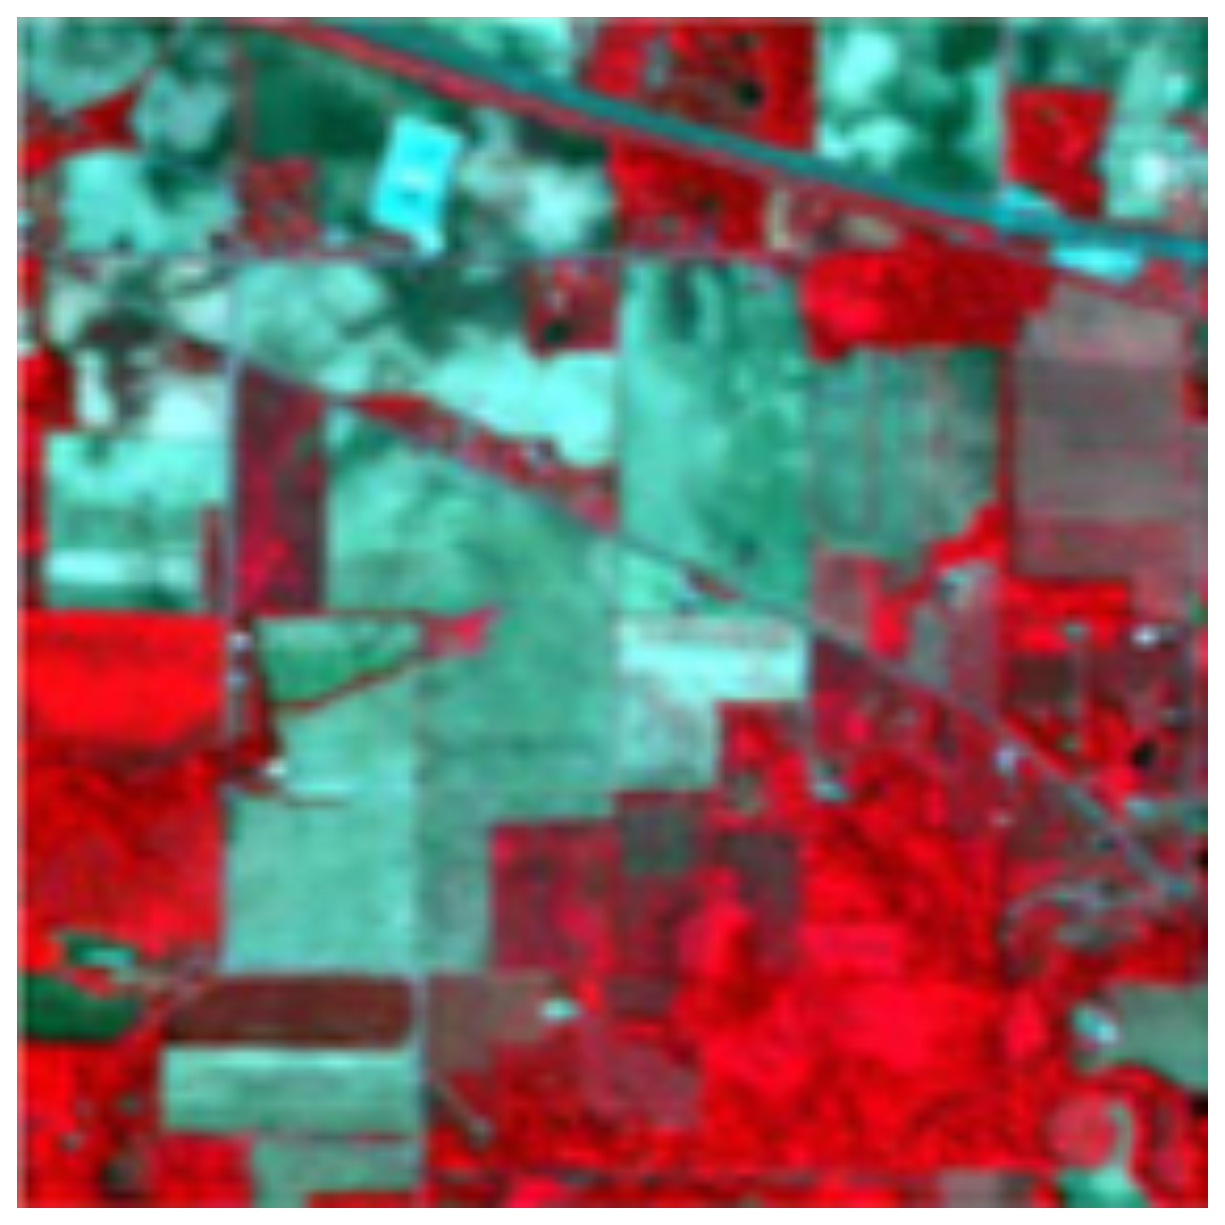
\includegraphics[height=2.4cm,width=2.4cm]{Figure/IN-FC.eps}
\end{minipage}
}
\subfigure[Truth Labels]{
\begin{minipage}[t]{0.14\textwidth}
\centering
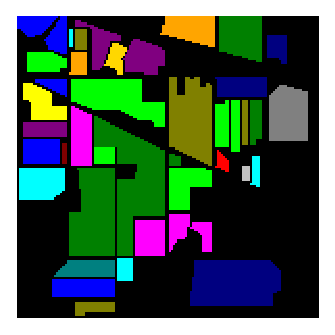
\includegraphics[height=2.4cm,width=2.4cm]{Figure/INlabels.eps}
\end{minipage}
}
\subfigure[3D-CNN]{
\begin{minipage}[t]{0.14\textwidth}
\centering
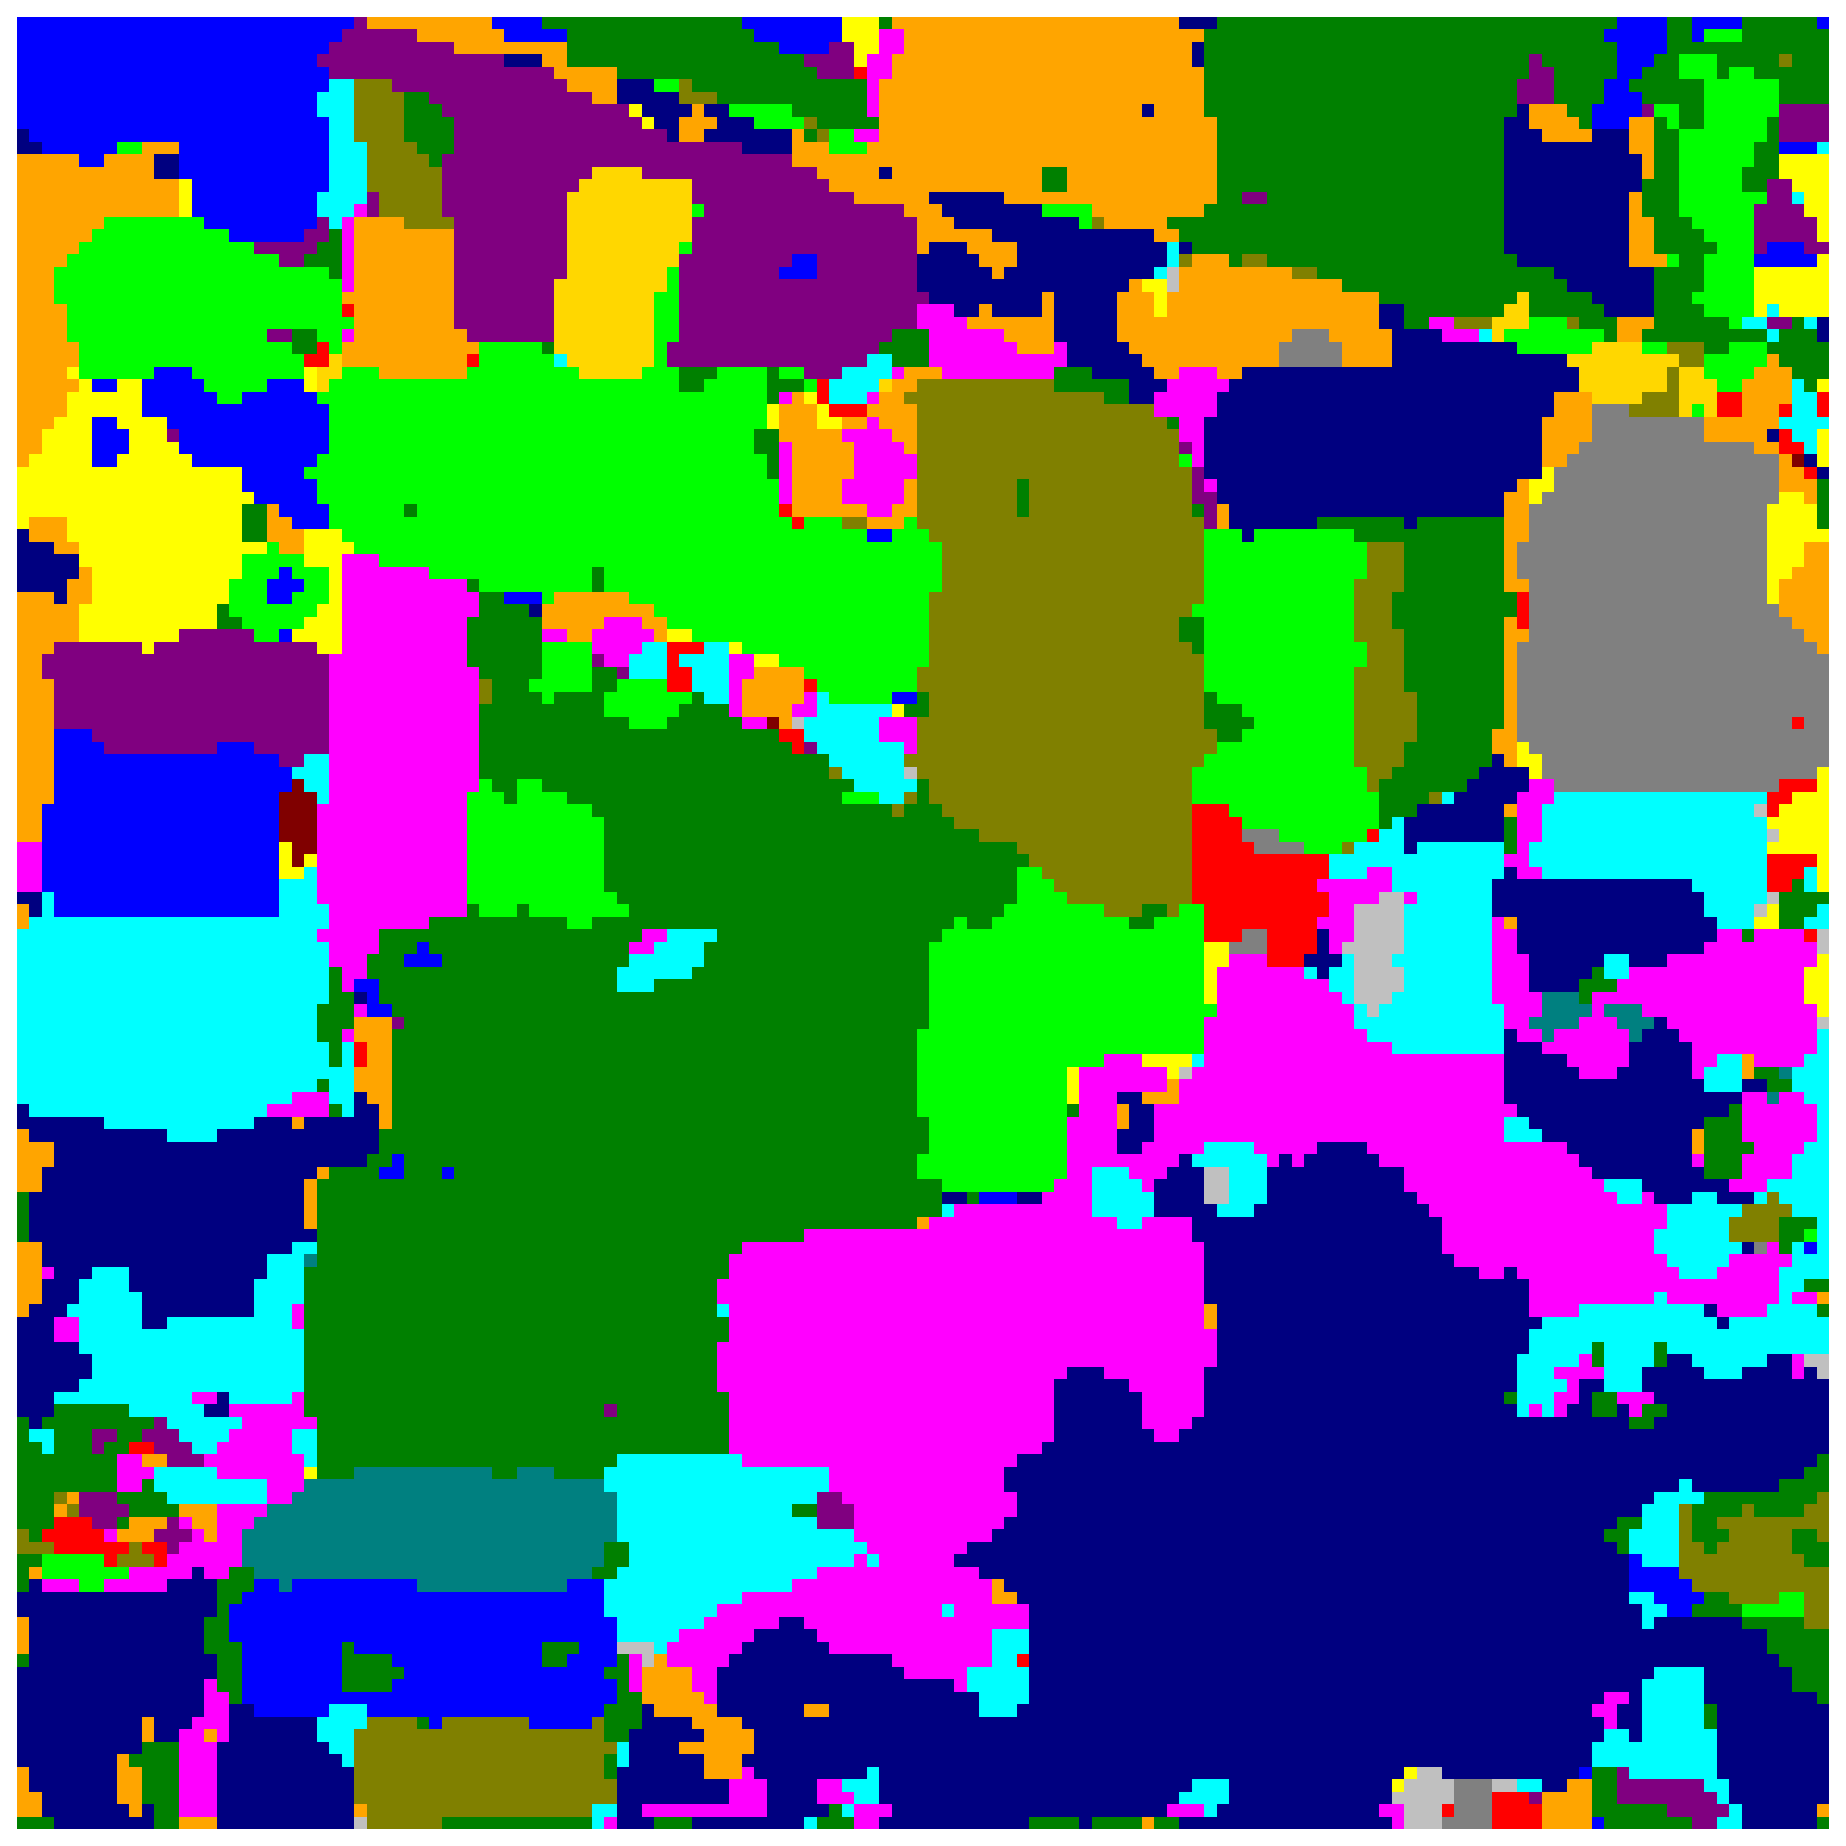
\includegraphics[height=2.4cm,width=2.4cm]{Figure/IN_3d.eps}
\end{minipage}
}
\subfigure[SSAN]{
\begin{minipage}[t]{0.14\textwidth}
\centering
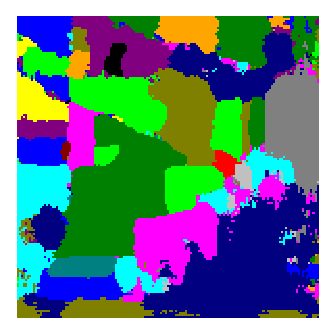
\includegraphics[height=2.4cm,width=2.4cm]{Figure/IN_SSAN.eps}
\end{minipage}
}
\subfigure[GCN]{
\begin{minipage}[t]{0.14\textwidth}
\centering
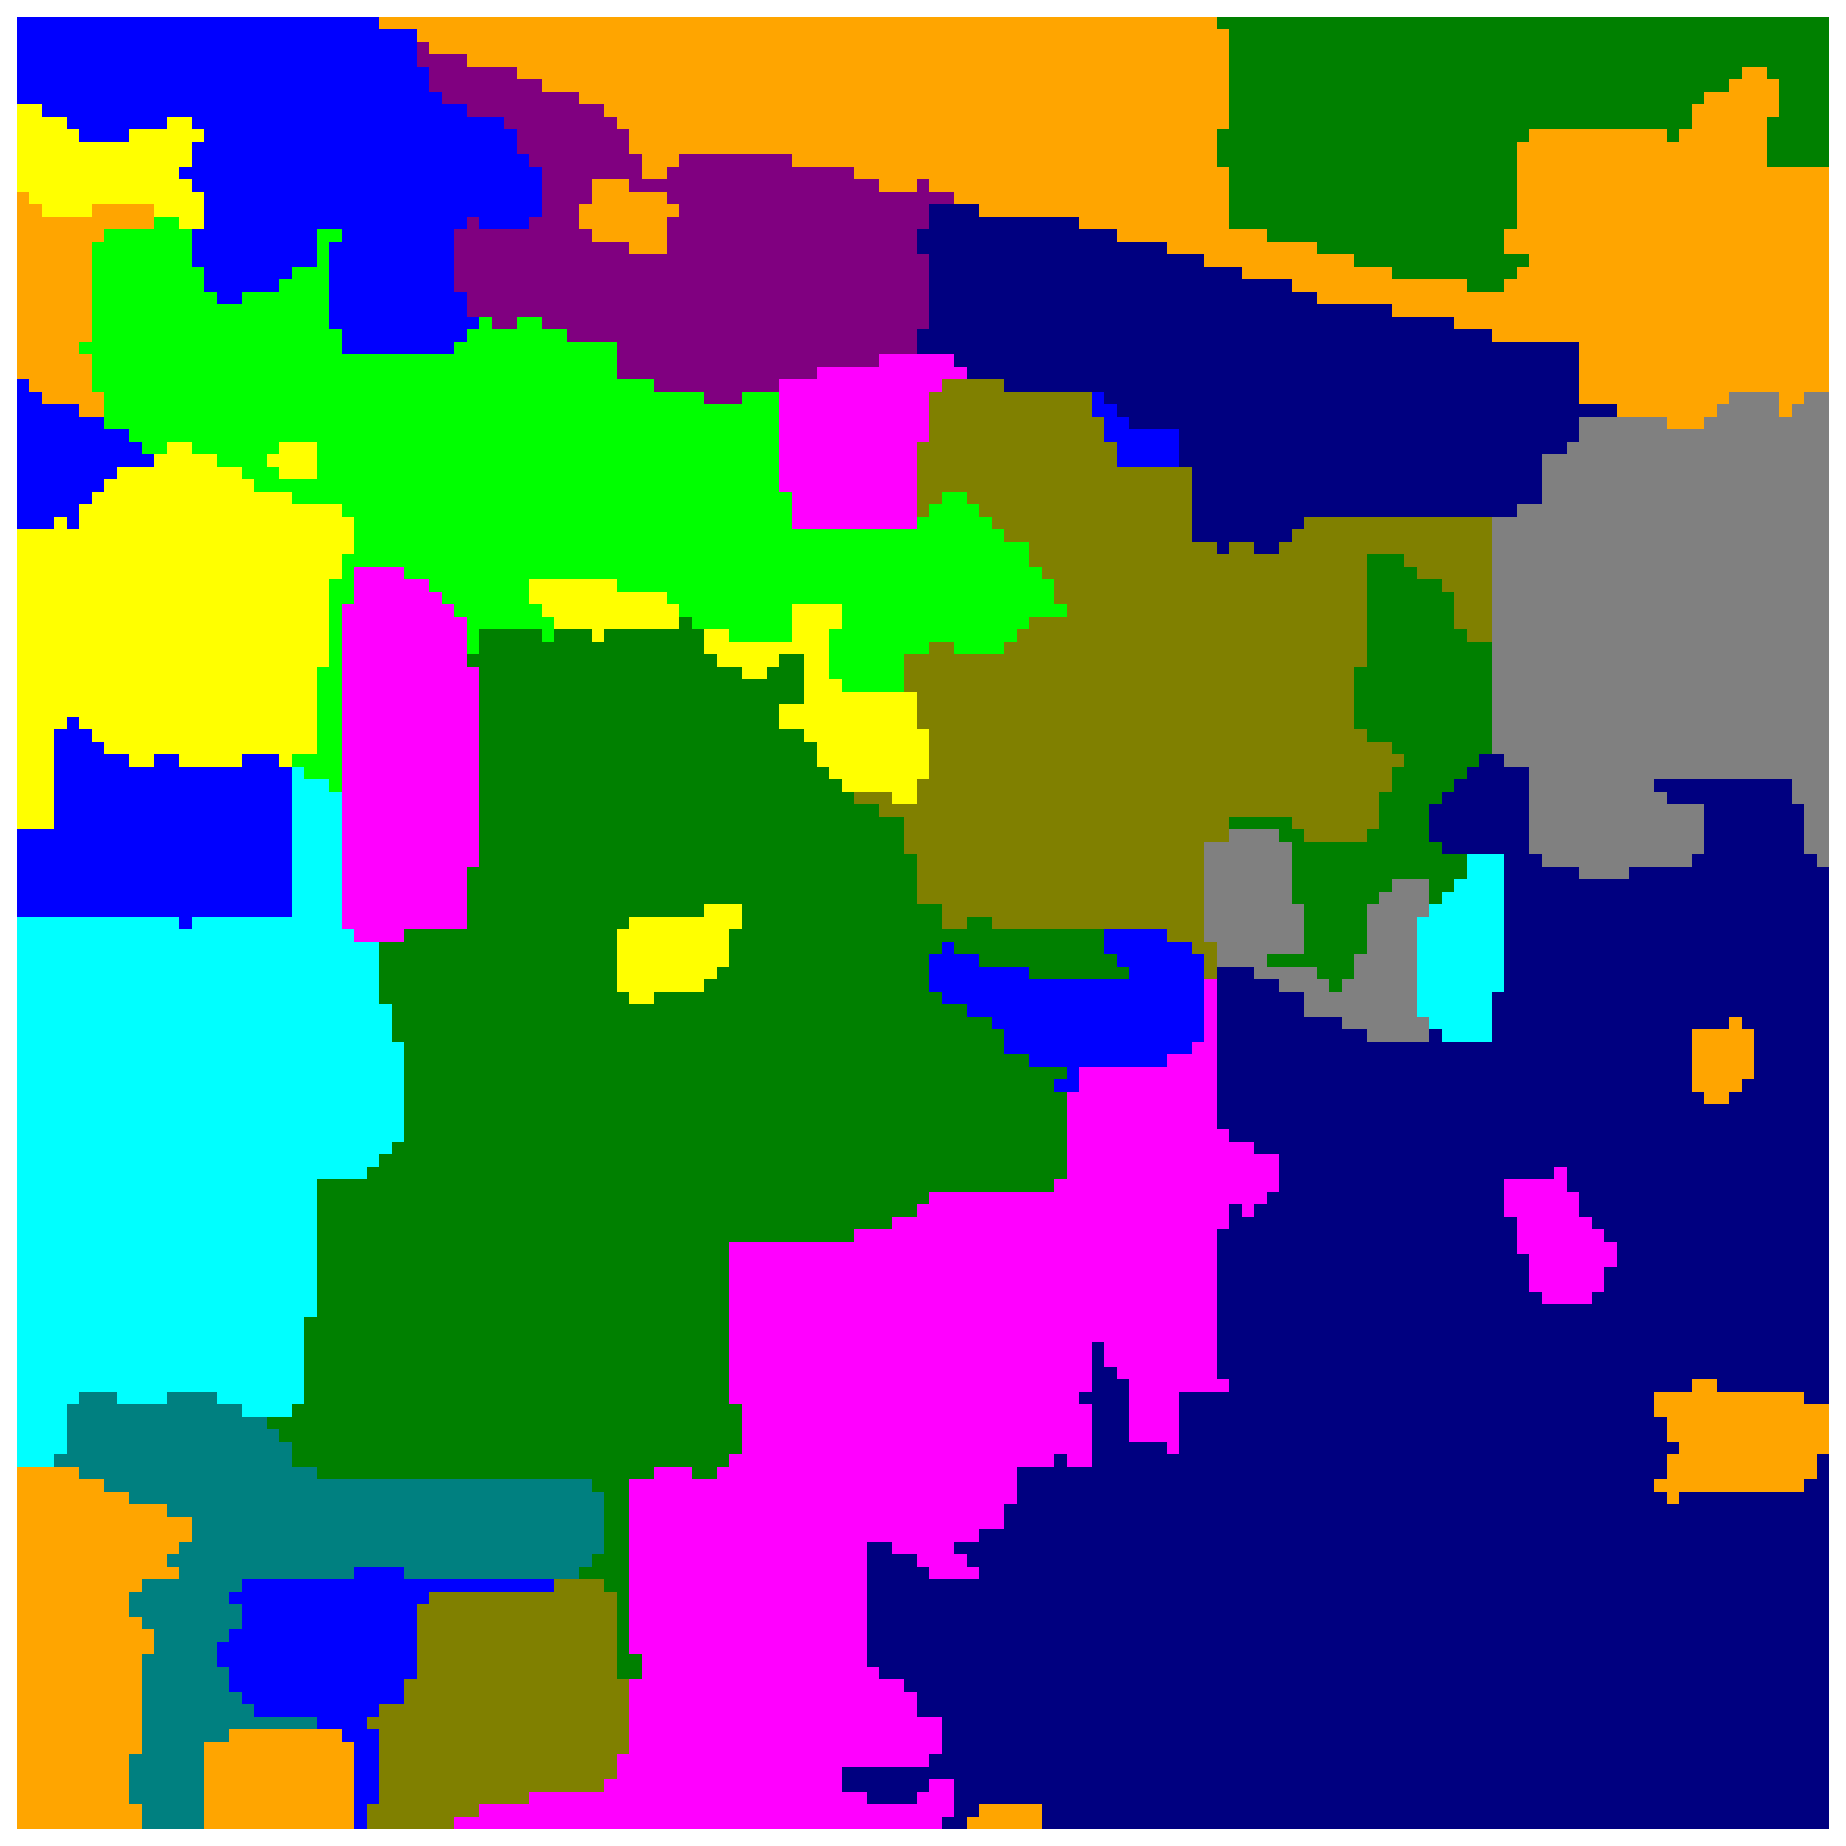
\includegraphics[height=2.4cm,width=2.4cm]{Figure/IN_GCN.eps}
\end{minipage}
}
\subfigure[SSRN]{
\begin{minipage}[t]{0.14\textwidth}
\centering
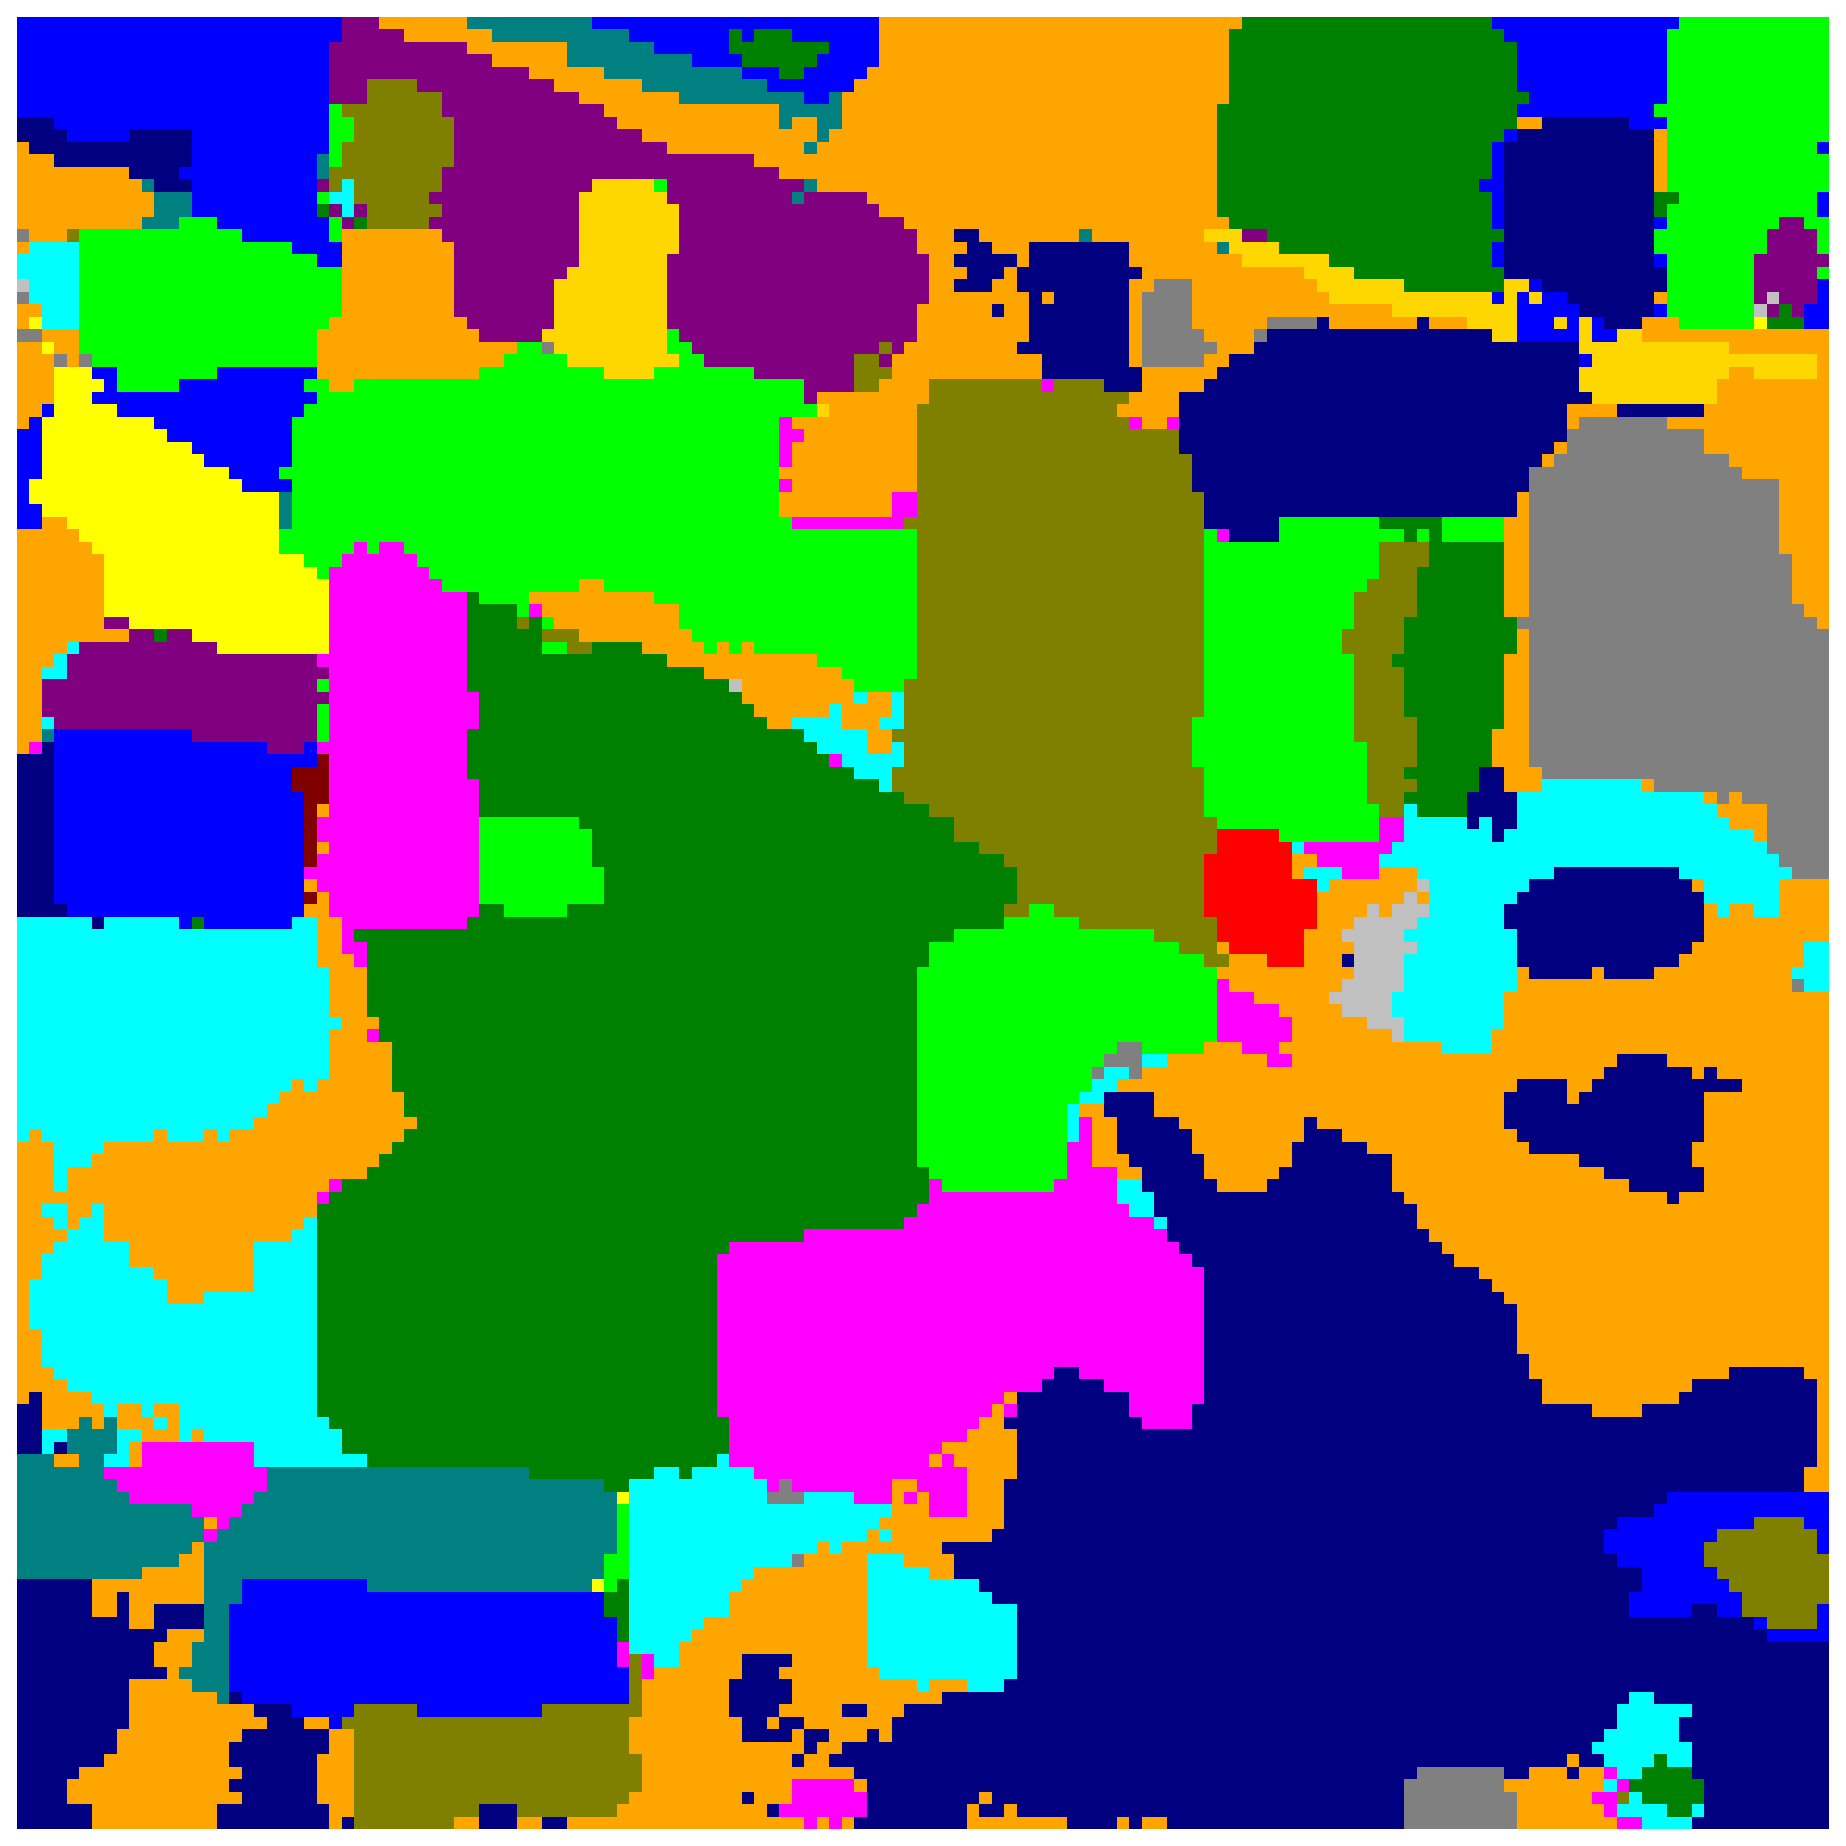
\includegraphics[height=2.4cm,width=2.4cm]{Figure/IN_SSRN.eps}
\end{minipage}
}
\subfigure[DenseNet]{
\begin{minipage}[t]{0.14\textwidth}
\centering
\includegraphics[height=2.4cm,width=2.4cm]{Figure/IN3Densenet.eps}
\end{minipage}
}
\subfigure[HybridSN]{
\begin{minipage}[t]{0.14\textwidth}
\centering
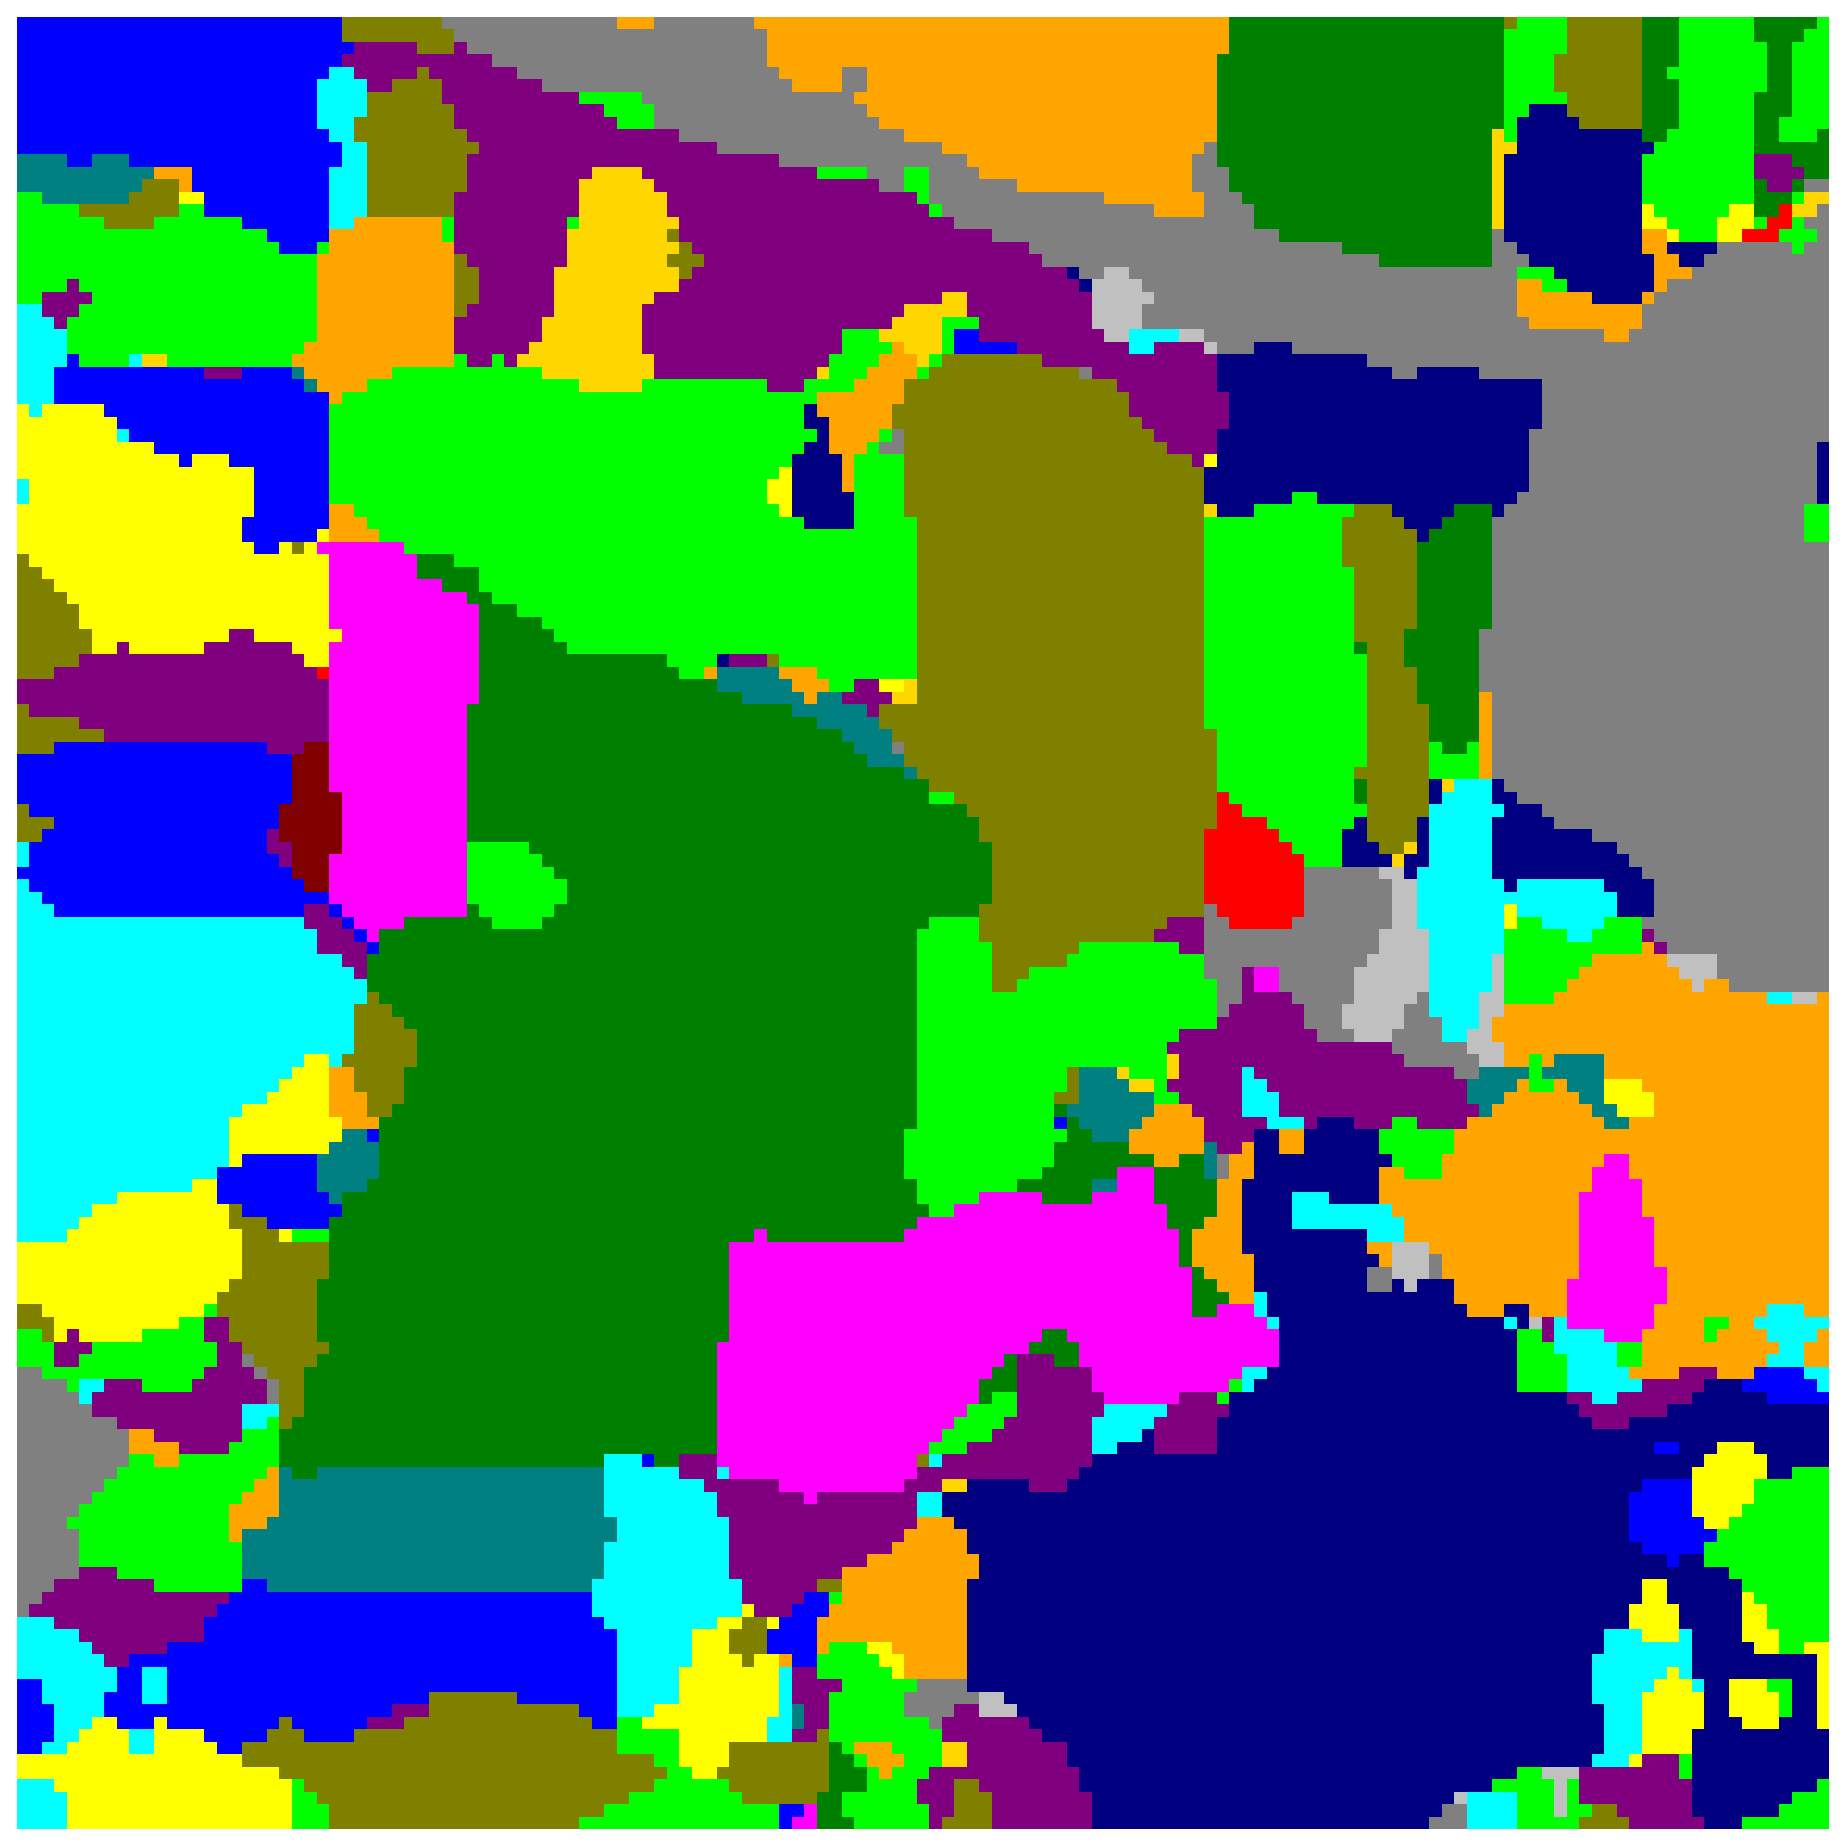
\includegraphics[height=2.4cm,width=2.4cm]{Figure/IN_HybridSN.eps}
\end{minipage}
}
\subfigure[SSFTT]{
\begin{minipage}[t]{0.14\textwidth}
\centering
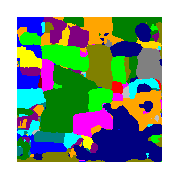
\includegraphics[height=2.4cm,width=2.4cm]{Figure/IN_SSFTT.eps}
\end{minipage}
}
\subfigure[Proposed]{
\begin{minipage}[t]{0.14\textwidth}
\centering
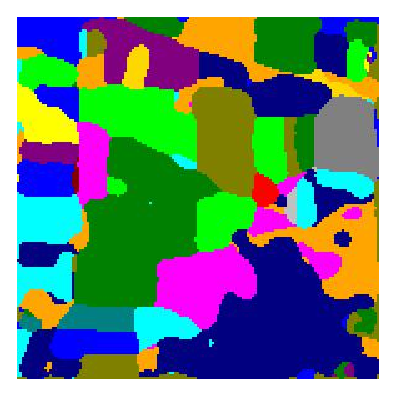
\includegraphics[height=2.4cm,width=2.4cm]{Figure/IN_proposed.eps}
\end{minipage}
}
\subfigure[Colors labels]{
\begin{minipage}[t]{0.14\textwidth}
\centering
\includegraphics[height=2.4cm,width=2.4cm]{Figure/IN_label.eps}
\end{minipage}
}

\caption{Classification maps of the most remarkable models of IN dataset with diverse methods.}\label{fig:5}
\end{figure*}
\graphicspath{{KSCfig/}}
\begin{figure*}[!htb]
\centering\small
\subfigure[False-color]{
\begin{minipage}[t]{0.14\textwidth}
\centering
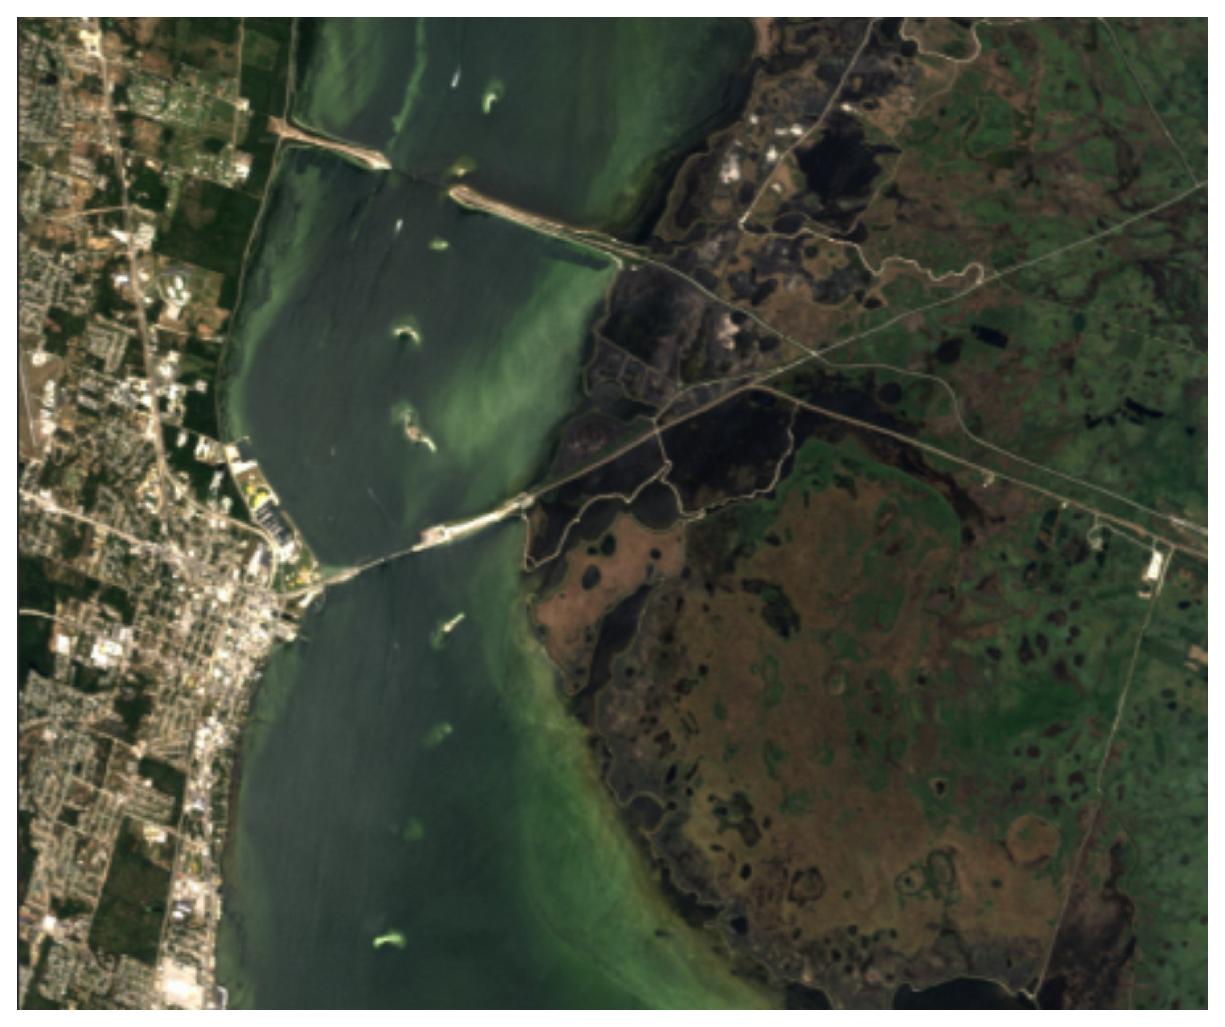
\includegraphics[height=2.4cm,width=2.4cm]{Figure/KSC-FC.eps}
\end{minipage}
}
\subfigure[Truth Labels]{
\begin{minipage}[t]{0.14\textwidth}
\centering
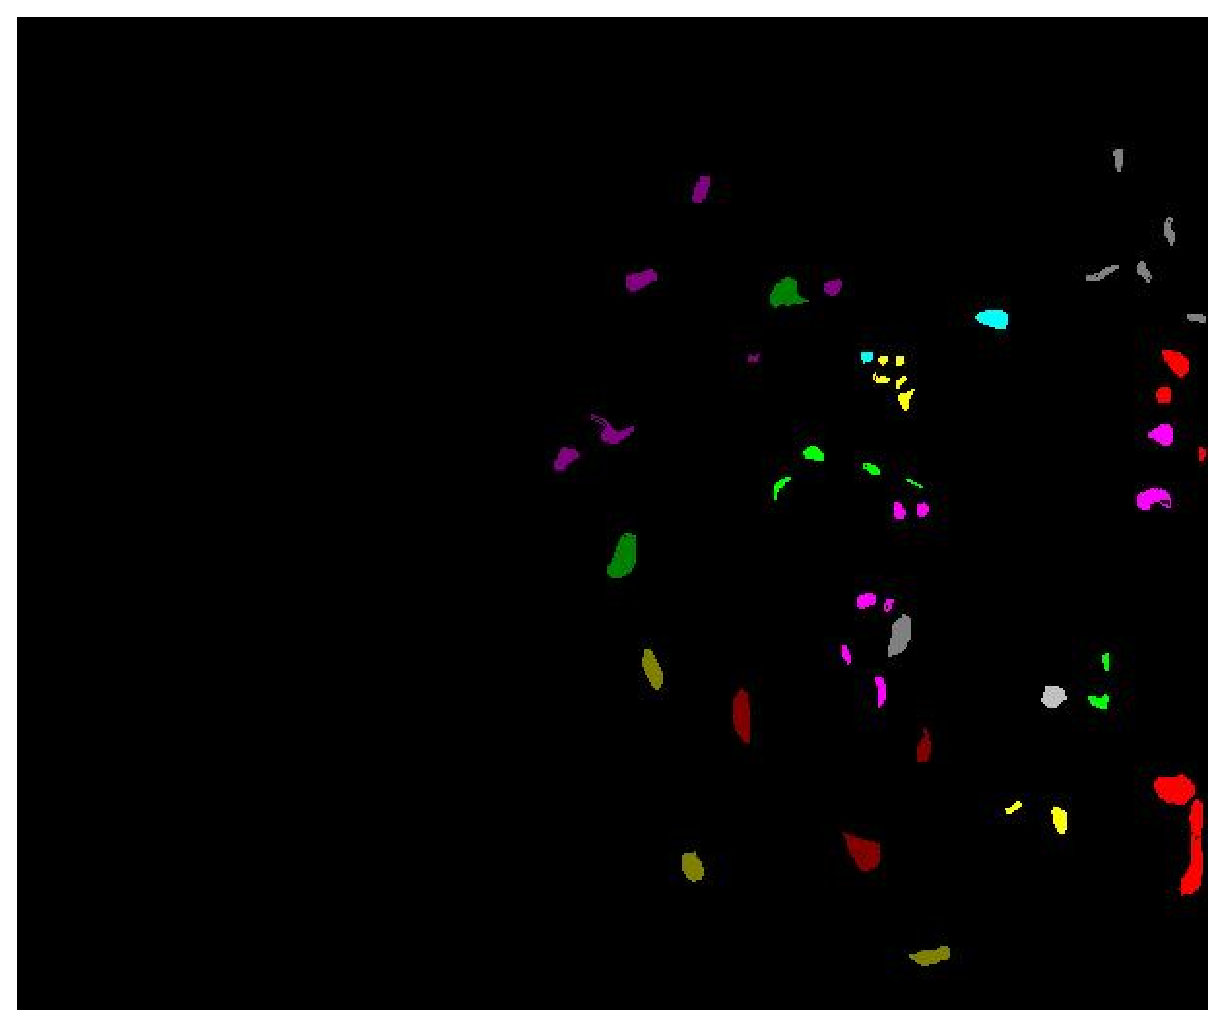
\includegraphics[height=2.4cm,width=2.4cm]{Figure/KSClabels.eps}
\end{minipage}
}
\subfigure[3D-CNN]{
\begin{minipage}[t]{0.14\textwidth}
\centering
\includegraphics[height=2.4cm,width=2.4cm]{Figure/ksc_3d.eps}
\end{minipage}
}
\subfigure[SSAN]{
\begin{minipage}[t]{0.14\textwidth}
\centering
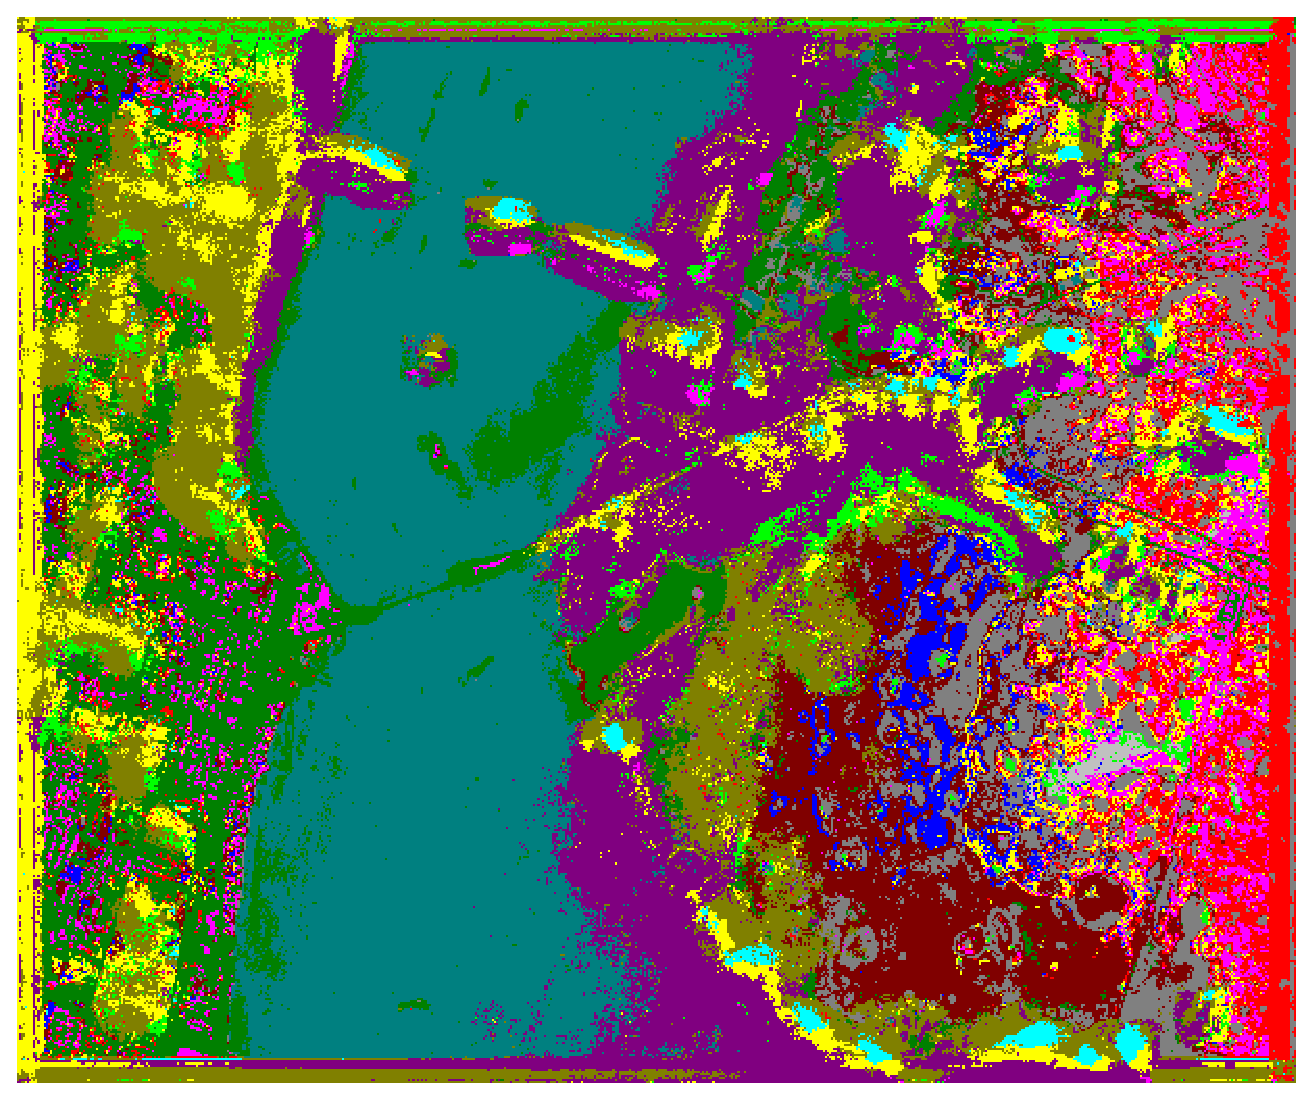
\includegraphics[height=2.4cm,width=2.4cm]{Figure/KSC_SSAN.eps}
\end{minipage}
}
\subfigure[GCN]{
\begin{minipage}[t]{0.14\textwidth}
\centering
\includegraphics[height=2.4cm,width=2.4cm]{Figure/KSC_GCN.eps}
\end{minipage}
}
\subfigure[SSRN]{
\begin{minipage}[t]{0.14\textwidth}
\centering
\includegraphics[height=2.4cm,width=2.4cm]{Figure/KSC_ssrn.eps}
\end{minipage}
}
\subfigure[DenseNet]{
\begin{minipage}[t]{0.14\textwidth}
\centering
\includegraphics[height=2.4cm,width=2.4cm]{Figure/KSC-3D_DenseNet.eps}
\end{minipage}
}
\subfigure[HybridSN]{
\begin{minipage}[t]{0.14\textwidth}
\centering
\includegraphics[height=2.4cm,width=2.4cm]{Figure/KSC_HybridSN.eps}
\end{minipage}
}
\subfigure[SSFTT]{
\begin{minipage}[t]{0.14\textwidth}
\centering
\includegraphics[height=2.4cm,width=2.4cm]{Figure/KSC_SSFTT.eps}
\end{minipage}
}
\subfigure[Proposed]{
\begin{minipage}[t]{0.14\textwidth}
\centering
\includegraphics[height=2.4cm,width=2.4cm]{Figure/KSC_proposed.eps}
\end{minipage}
}
\subfigure[Colors labels]{
\begin{minipage}[t]{0.14\textwidth}
\includegraphics[height=2.4cm,width=2.4cm]{Figure/KSC_label.eps}
\end{minipage}
}

\caption{Classification maps of the most remarkable models of KSC dataset with diverse methods.}\label{fig:6}
\end{figure*}
\graphicspath{{UPfig/}}
\begin{figure*}[!htb]
\centering\small
\subfigure[False-color]{
\begin{minipage}[t]{0.14\textwidth}
\centering
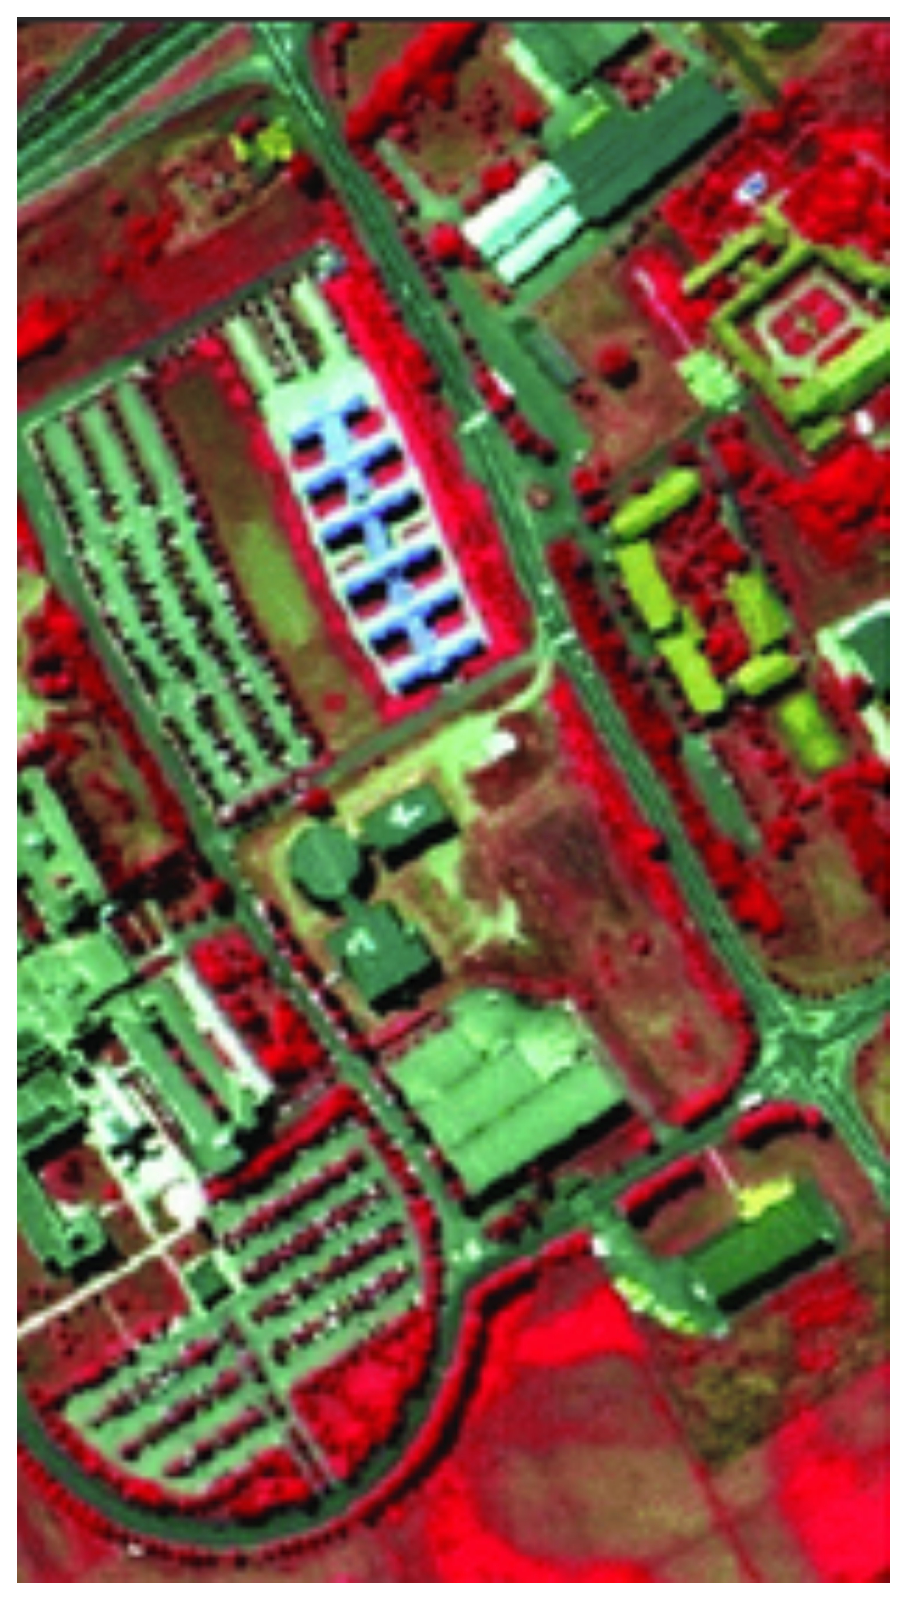
\includegraphics[height=4cm,width=2.4cm]{Figure/UP-FC.eps}
\end{minipage}
}
\subfigure[Truth Labels]{
\begin{minipage}[t]{0.14\textwidth}
\centering
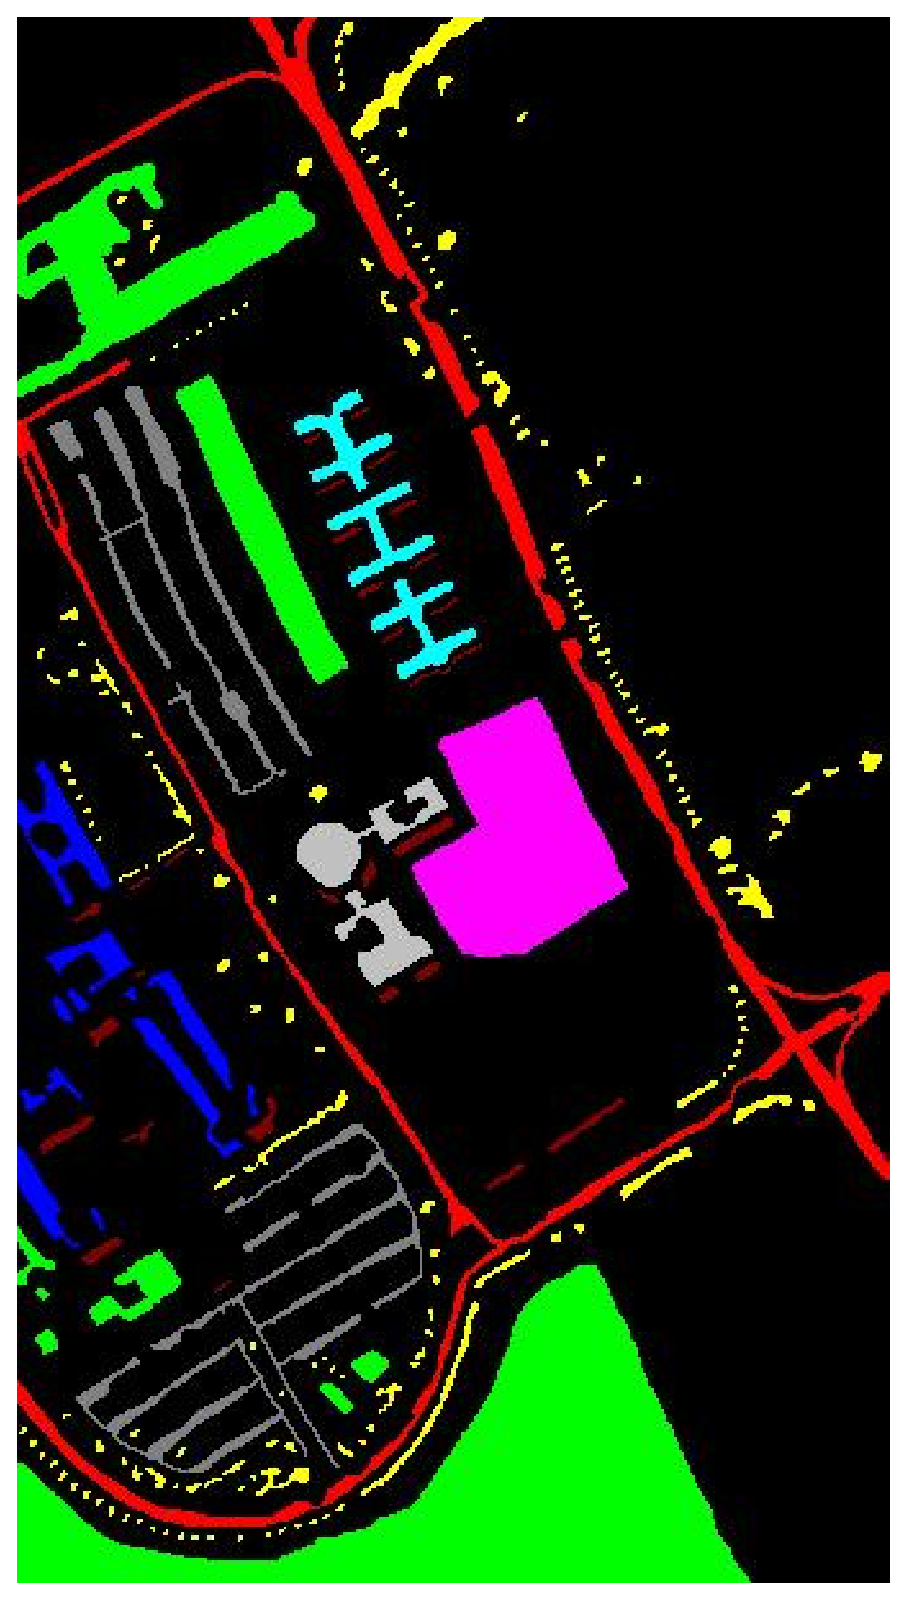
\includegraphics[height=4cm,width=2.4cm]{Figure/UPlabels.eps}
\end{minipage}
}
\subfigure[3D-CNN]{
\begin{minipage}[t]{0.14\textwidth}
\centering
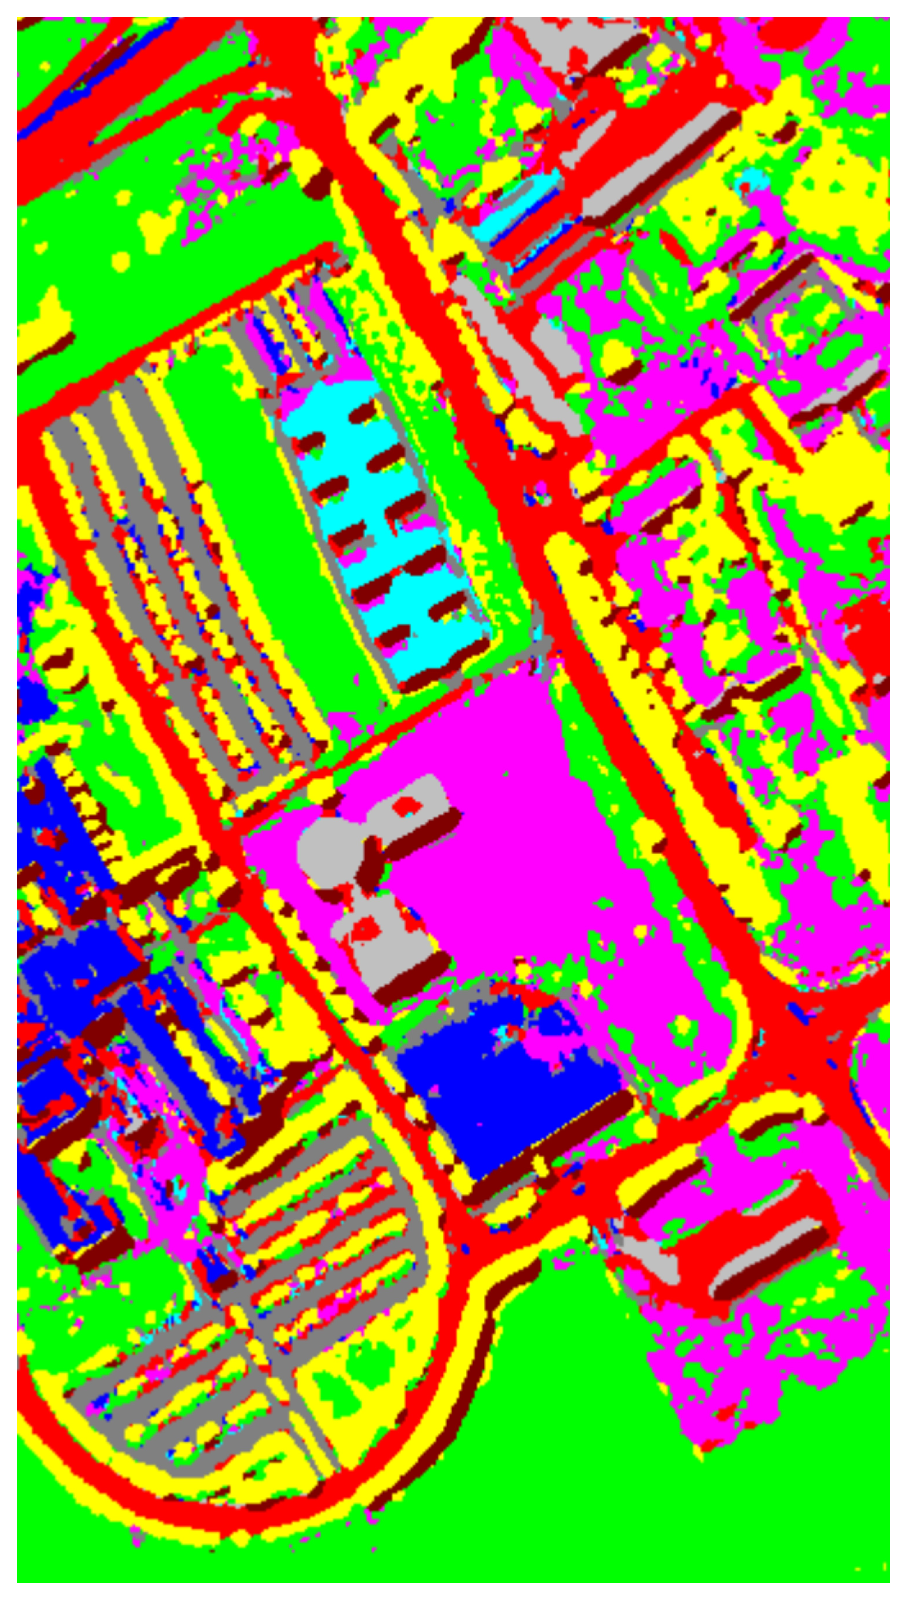
\includegraphics[height=4cm,width=2.4cm]{Figure/UP_3d.eps}
\end{minipage}
}
\subfigure[SSAN]{
\begin{minipage}[t]{0.14\textwidth}
\centering
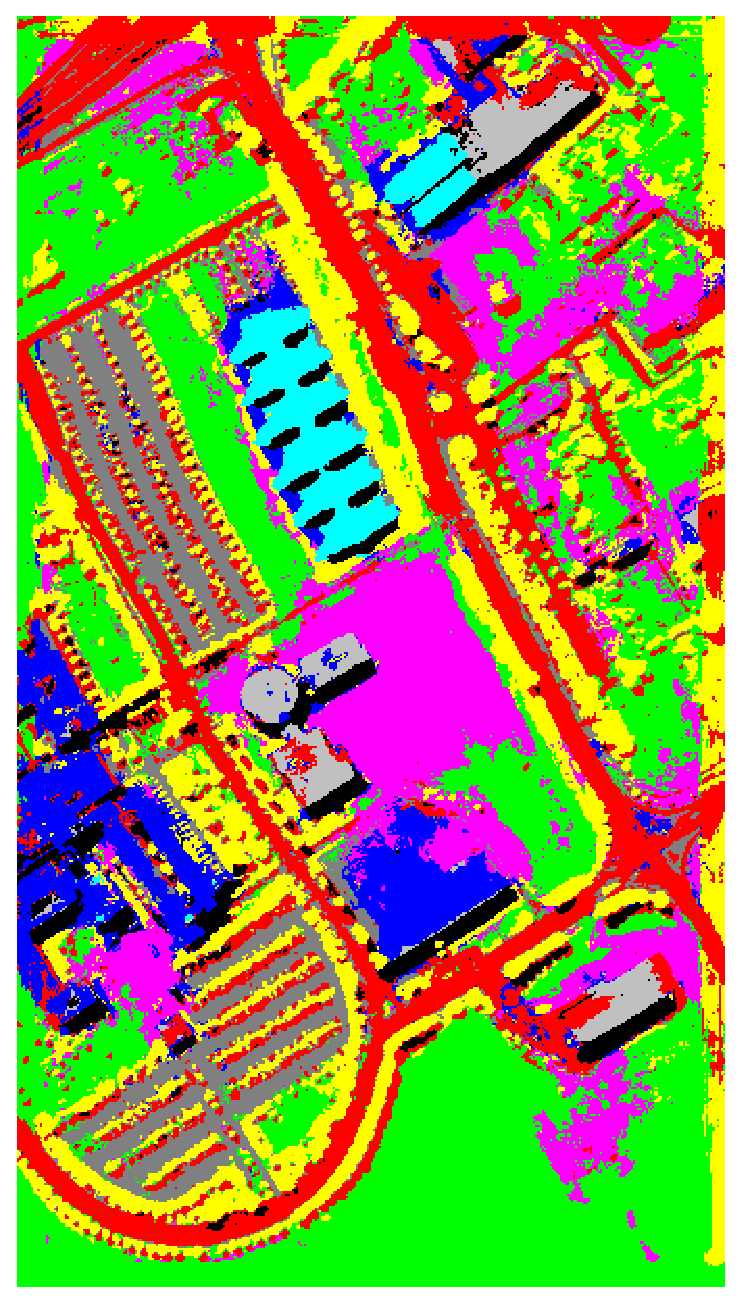
\includegraphics[height=4cm,width=2.4cm]{Figure/UP_SSAN.eps}
\end{minipage}
}
\subfigure[GCN]{
\begin{minipage}[t]{0.14\textwidth}
\centering
\includegraphics[height=4cm,width=2.4cm]{Figure/UP_gcn.eps}
\end{minipage}
}
\subfigure[SSRN]{
\begin{minipage}[t]{0.14\textwidth}
\centering
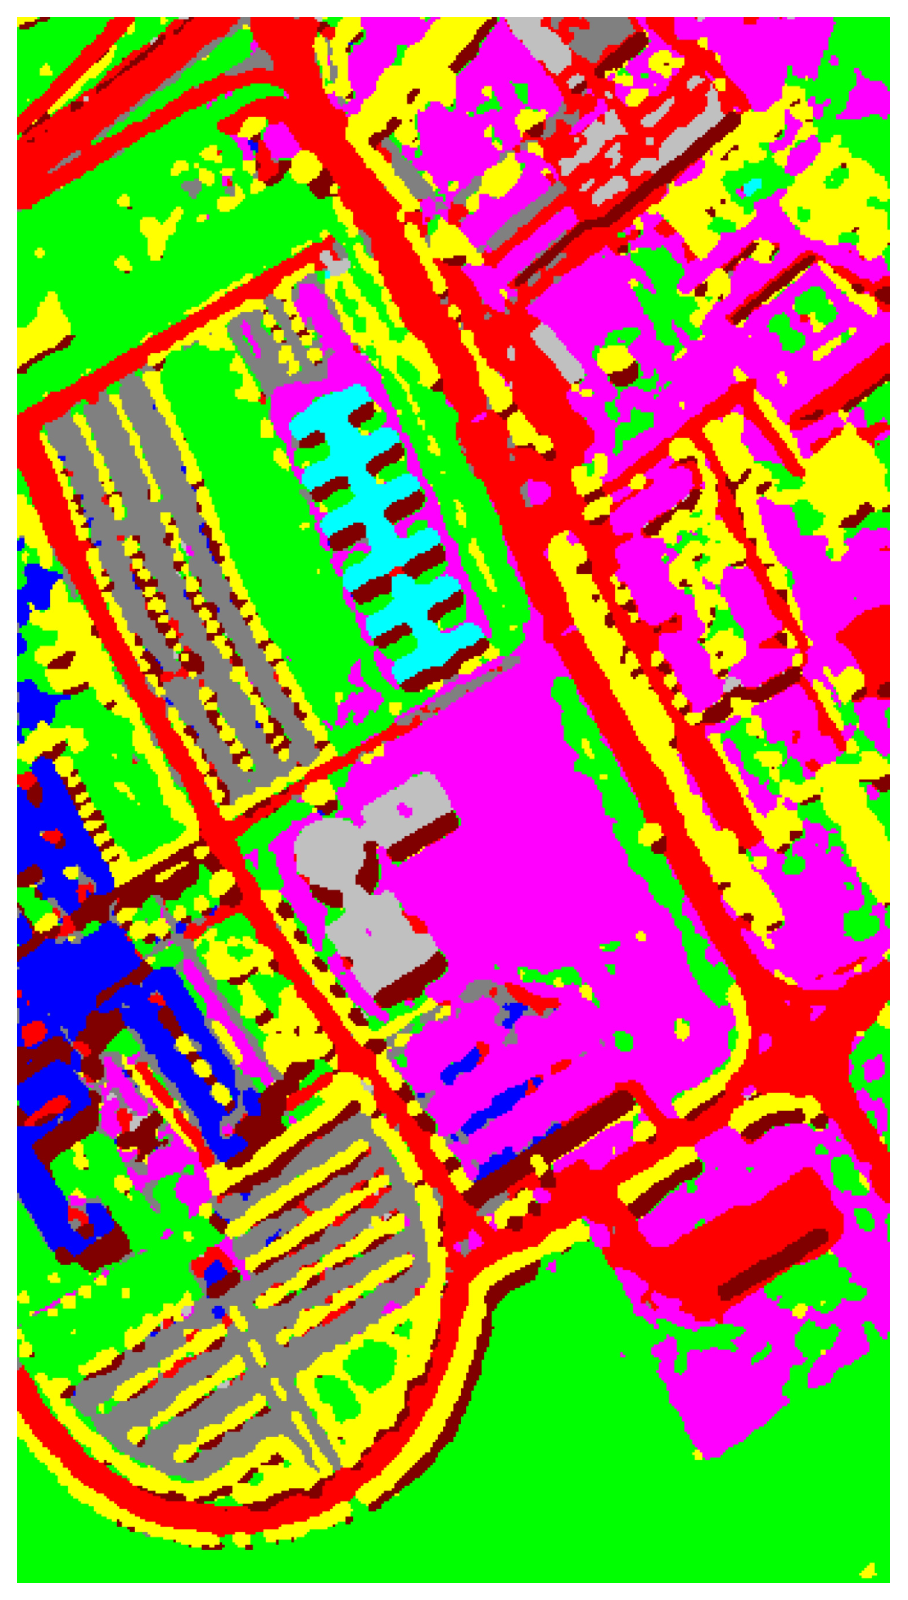
\includegraphics[height=4cm,width=2.4cm]{Figure/UP_SSRN.eps}
\end{minipage}
}
\subfigure[DenseNet]{
\begin{minipage}[t]{0.14\textwidth}
\centering
\includegraphics[height=4cm,width=2.4cm]{Figure/UP-3D-DenseNet.eps}
\end{minipage}
}
\subfigure[HybridSN]{
\begin{minipage}[t]{0.14\textwidth}
\centering
\includegraphics[height=4cm,width=2.4cm]{Figure/UP_HybridSN.eps}
\end{minipage}
}
\subfigure[SSFTT]{
\begin{minipage}[t]{0.14\textwidth}
\centering
\includegraphics[height=4cm,width=2.4cm]{Figure/UP_SSFTT.eps}
\end{minipage}
}
\subfigure[Proposed]{
\begin{minipage}[t]{0.14\textwidth}
\centering
\includegraphics[height=4cm,width=2.4cm]{Figure/UP_proposed.eps}
\end{minipage}
}
\subfigure[Colors labels]{
\begin{minipage}[t]{0.14\textwidth}
\centering
\includegraphics[height=4cm,width=2.4cm]{Figure/UP_label.eps}
\end{minipage}}
\caption{Classification maps of the most remarkable models of UP dataset with diverse methods.}\label{fig:7}
\end{figure*}

\section{Discussion and Analysis}
A patch block of size $S\times S\times B$, where $S$ stands for the space size and $B$ for the primary component, is the input to the MPSSAN network. We will examine each one's impact on categorization performance independently in the sections that follow. In each of the three datasets, we ran tests with $B$ fixed at $30$ and spatial sizes ranging from $13$ to $21$, as seen in Figure \ref{fig:8}(a), When we feed the network with increasingly accurate data, the experimental findings demonstrate that accuracy rises as the spatial size grows. Larger is not necessarily better, and the noise that comes along with more useful information adds to the expense of training. Finally, we settled on spatial sizes of $21\times 21$ on the KSC dataset and $17\times 17$ on the IN and UP datasets.

Figure \ref{fig:8}(b) displays the OA on the three datasets using different number of principal components and the selected optimum space size. The deeper information input into our network architecture is the reason why the overall accuracy tends to gradually rise with the number of major components.
The results of the present study indicate that when the principal component is greater than $20$, the overall accuracy of UP declines, in contrast to the datasets IN and KSC. As can be seen, the best results are obtained when the KSC dataset and IN dataset are set to $40$ and the UP dataset  is set to $20$. When the best results were obtained, we performed the experiment as depicted in Figure \ref{fig:8}(c), fixing the total  number of principal components, breaking the original hyperspectral data into a number of groups, and extracting several principal components from each group. We fixed $40$ principal components and performed five sets of ablation experiments; in other words, $40$ principal components were directly extracted from the entire original hyperspectral image, and the original image was split into two groups by bands, with $20$ principal components being extracted from each group, respectively. Ten primary components were taken from each of the four groups. The image was split into $8$ groups, each of which included $5$ principal components, and $5$ groups, each of which contained $8$ principal components. It was discovered that for the IN dataset, the highest accuracy was obtained when it was divided into $5$ groups, and $8$ principal components were extracted from each group. While OA and Kappa are not much impacted by this, AA swings widely and may be affected by the correlation of nearby bands.

\begin{figure*}[h]
\subfigure[]{
\begin{minipage}[t]{0.3\textwidth}
\centering
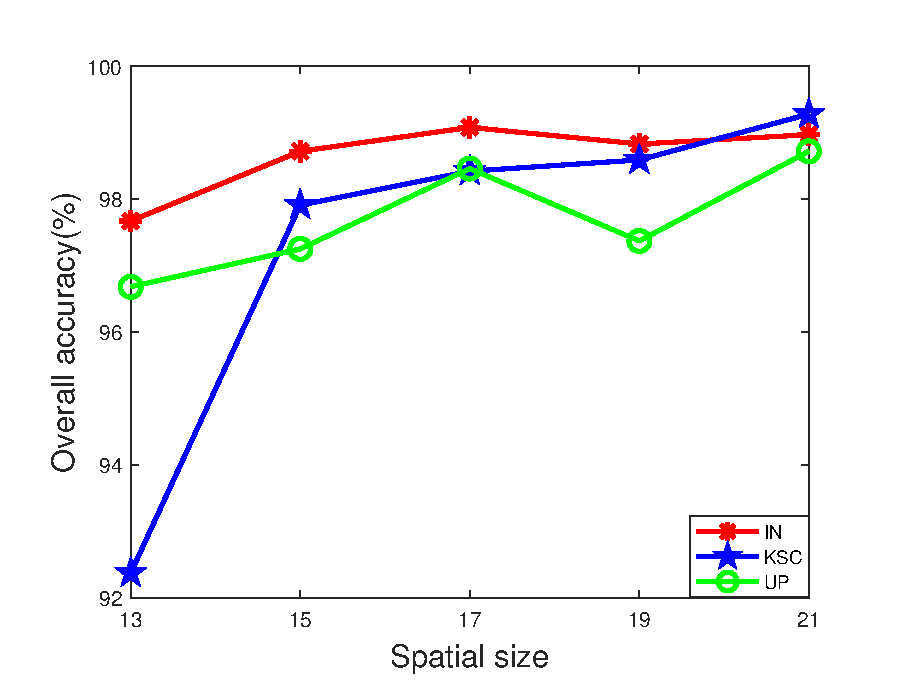
\includegraphics[height=3.8cm,width=4.9cm]{Spatial.eps}
\end{minipage}
}
\subfigure[]{
\begin{minipage}[t]{0.3\textwidth}
\centering
\includegraphics[height=3.8cm,width=4.9cm]{pca.eps}
\end{minipage}
}
\subfigure[]{
\begin{minipage}[t]{0.3\textwidth}
\centering
\includegraphics[height=3.8cm,width=4.9cm]{groups.eps}
\end{minipage}
}
\caption{Effect of spatial sizes and principal components on three datasets.}
\label{fig:8}
\end{figure*}

We trained the IN and KSC datasets using 5\%, 10\%, 15\%, and 20\% samples, respectively, to see how the quantity of training samples influenced our model architecture and several other methods. We just used training samples of 0.5\%, 1\%, 1.5\%, and 2\% because the UP dataset with labeled samples is adequate. We select an input size of $17 \times 17 \times 40$ for the IN dataset, train the KSC dataset using samples under the condition of $21 \times 21 \times 40$, and select an input size of $17 \times 17 \times 20$ for the UP dataset. On the IN and KSC datasets, the overall accuracy is 96.87\% and 98.14\%, respectively, when the sample size is 5\%. The overall accuracy of the UP dataset is 95.67\% when the sample size is 0.5\%. As can be seen in Figure \ref{fig:9}, the model performance keeps improving as the number of samples increases, and the accuracy is between 99\% and 100\% when the number of samples is enough. The studies demonstrate that our model can still classify objects accurately even with a small number of labeled samples. They also show that a multi-scale architecture can successfully classify objects using joint spectral and spatial information.
\begin{figure*}[!h]
\centering\small
\subfigure[IN]{
\begin{minipage}[t]{0.3\textwidth}
\centering
\includegraphics[height=3.8cm,width=5cm]{samples-IN.eps}
\end{minipage}
}
\subfigure[KSC]{
\begin{minipage}[t]{0.3\textwidth}
\centering
\includegraphics[height=3.8cm,width=5cm]{samples-KSC.eps}
\end{minipage}
}
\subfigure[UP]{
\begin{minipage}[t]{0.3\textwidth}
\centering
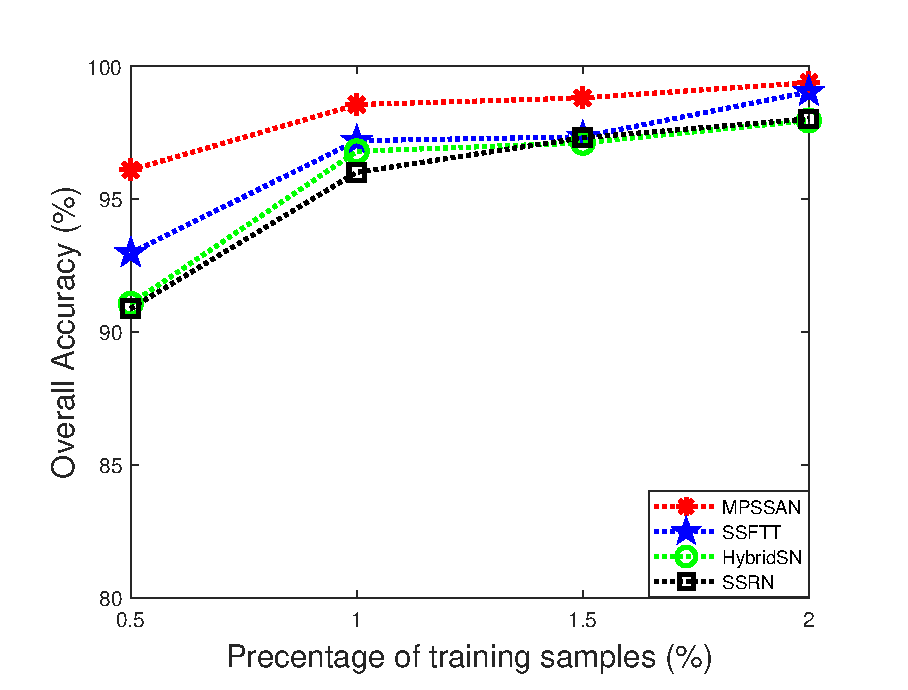
\includegraphics[height=3.8cm,width=5cm]{samples-UP.eps}
\end{minipage}
}
\caption{Overall accuracy with different training samples on three datasets.}\label{fig:9}
\end{figure*}


To test the efficacy of DSACM, we conducted two sets of experiments on three datasets, one with and one without the DSACM module. The results of the experiments are displayed in Figure \ref{fig:10}(a). The performance of the model is enhanced because DSACM not only concentrates on the spectral features of hyperspectral images but also incorporates spatial features into the attention mechanism to better convey the prominent features of hyperspectral images. We separated 3D convolution into two separate modules: Spectral feature extraction and spatial feature extraction. We conducted three sets of tests on three different datasets to prove the value of the two sections, and the results are displayed in Figure \ref{fig:10}(b). The spectral-spatial joint extraction yields the best results, followed by the spatial feature extraction module by itself. Therefore, we should make full use of the spectral and spatial information as much as possible in the hyperspectral feature extraction.



\begin{figure*}[!h]
\centering\small
\subfigure[]{
\begin{minipage}[t]{0.48\textwidth}
\centering
\includegraphics[height=4.8cm,width=7cm]{DSACM-analyse.eps}
\end{minipage}
}
\subfigure[]{
\begin{minipage}[t]{0.48\textwidth}
\centering
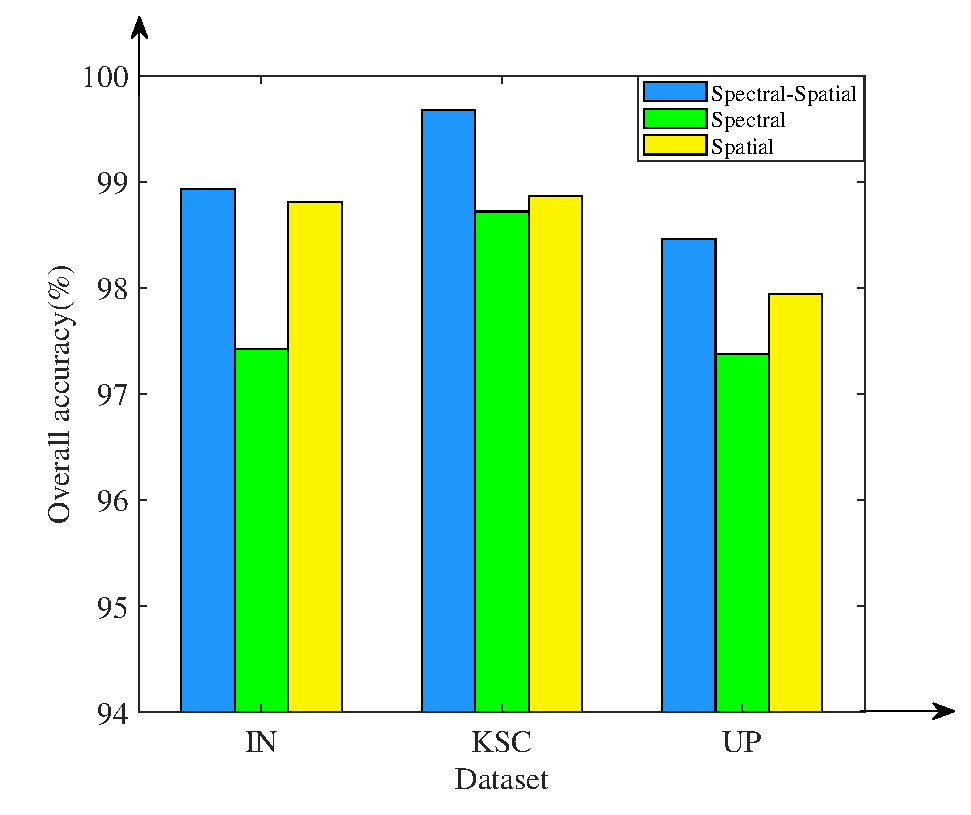
\includegraphics[height=4.8cm,width=7cm]{spectral-spatial.eps}
\end{minipage}
}

\caption{Impact of different modules on three datasets.}\label{fig:10}
\end{figure*}






\section{Conclusion and Future Works}

The fundamental advantage of the presented model is its simple structure, which extracts more discriminative properties through the simple convolution of many layers. The multi-scale idea is used to grow the network, as opposed to the redundant network layers of ResNet and DenseNet in the past. Despite the high level of duplication in the original data, we continue to use the principal component analysis method and sub-band for dimensionality reduction. The MPSSAN network fully utilizes the advantages of both 2D and 3D convolution to extract both spectral and spatial data sequentially. With DSACM, useful traits are emphasized while erroneous information is suppressed. The probability values are finally forecasted using LogSoftmax. Results from three frequently used datasets show how well our proposed network design classifies data. Our next objective is to look into a more logical and scientific division because we currently use random division for band division. We also need to investigate more effective attention modules to improve network performance in the future.


\section*{Disclosure statement}

No potential conflict of interest was reported by the authors.

\section*{Funding}

This research was supported by the National Natural Science Foundation of China under Grant No.62072468.
\bibliographystyle{tfcad}
\bibliography{interactcadsample}
\end{document}
